\documentclass[10pt,a4paper,twocolumn]{article}
\usepackage[margin=1.75cm,columnsep=0.65cm]{geometry}
\usepackage[T1]{fontenc}
\usepackage[utf8]{inputenc}
\usepackage{amsmath}
% newtxmath supplies its own symbol definitions; do not load amssymb after it.
\IfFileExists{newtxtext.sty}{\usepackage{newtxtext,newtxmath}}{\usepackage{mathptmx}}
\usepackage{microtype}
\usepackage{graphicx}
\usepackage{booktabs,tabularx,array,multirow}
\usepackage{arydshln}
\usepackage{caption,float}
\usepackage[section]{placeins}
\usepackage{etoolbox}
\usepackage{tikz}
\usetikzlibrary{positioning,arrows.meta,shapes.geometric}
\usepackage{dblfloatfix}
\pretocmd{\subsection}{\FloatBarrier}{}{\PackageError{report}{Cannot install subsection float barriers}{}}
\usepackage[numbers,sort&compress]{natbib}
\usepackage[hidelinks]{hyperref}
\usepackage{siunitx}
\sisetup{
    group-separator = {\,},
    group-minimum-digits = 4
}
\hypersetup{pdftitle={Waveform-based timing correction for time-of-flight positron emission tomography}, pdfauthor={Alessandro Falcetta}}
\captionsetup{font=small,labelfont=bf}
\setlength{\emergencystretch}{1.5em}
\newcommand{\placeholder}[1]{\par\noindent\textit{[Placeholder: #1]}\par}
\newcommand{\figureplaceholder}[2]{%
  \begin{figure}[tbp]\centering
  \fbox{\begin{minipage}[c][2.3cm][c]{0.92\columnwidth}\centering
  \textit{Placeholder: #1.}\end{minipage}}
  \caption{#1.}\label{#2}
  \end{figure}}
\title{Waveform-based timing correction for time-of-flight positron emission tomography}
\author{Alessandro Falcetta}
\date{}
\begin{document}
\maketitle

\begin{abstract}
Accurate coincidence timing is essential for time-of-flight positron emission tomography. 
This study investigates machine-learning corrections to leading-edge timing using waveforms 
from two amplification stages and two readout boards, comparing different estimators, 
detector-shared formulations, and waveform windows.

Waveform-based correction improves first-stage coincidence timing resolution (CTR) by over $20\%$, 
reaching approximately $25\%$ with extended windows. Linear models perform competitively with neural networks, 
while detector-shared estimators retain most of the achievable correction. 
Wider windows reveal useful timing information beyond the leading edge. 
Nevertheless, second-stage signals remain superior, achieving corrected CTRs 
of approximately $53\,\mathrm{ps}$.
\end{abstract}

\section{Introduction}
Positron emission tomography (PET) detects pairs of annihilation photons to reconstruct
radiotracer distributions. Time-of-flight (TOF) information uses the difference between
photon arrival times to constrain the annihilation position along the line joining the
detectors and can improve image signal-to-noise performance. The precision of this
information depends on the coincidence timing resolution (CTR), conventionally expressed
as the full width at half maximum (FWHM) of the time-difference distribution~\cite{surti2015}.

A leading-edge discriminator (LED) assigns an arrival time when a pulse crosses a fixed
amplitude threshold. Variations in pulse amplitude and rising-edge shape shift the crossing
time, producing time walk. Digitized waveforms retain information about these variations,
which machine learning (ML) can exploit to estimate event-specific timing corrections.

Waveform-based approaches include direct TOF estimation and correction of conventional
timing measurements. Berg and Cherry demonstrated direct TOF estimation from detector
waveform pairs using a convolutional neural network (CNN), improving CTR by 20\% relative
to LED, from 231 to 185 ps~\cite{berg2018}. Onishi et al. combined LED with a CNN
trained using waveforms acquired at a single source position, improving timing
resolution while avoiding the position-dependent bias associated with direct TOF
estimation~\cite{onishi2022}. Feng et al. explored convolutional features combined with
transformer-based attention to capture local and global temporal information~\cite{feng2024}.
For bismuth germanate (BGO) detectors, Loignon-Houle et al. compared LED, a
two-threshold time-walk correction and CNN-based timing, showing that performance gains
and timing-distribution tails depend on detector characteristics~\cite{loignon2025}.

An open question is whether waveform samples beyond the rising edge improve
ML-based LED timing corrections, and which temporal regions contribute most.
Previous CNN studies have primarily examined short windows near the rising
edge~\cite{onishi2022,loignon2025}, leaving extended-window performance at high
sampling rates insufficiently characterized. In related model-based work,
Ruiz-Gonzalez et al. observed diminishing returns from additional samples
and found that the advantage of maximum-likelihood timing over digital
discrimination disappeared above 2 GS/s~\cite{ruiz2018}. These results do
not establish whether extending the waveform window benefits data-driven
corrections at the 80 GS/s acquisition rate used here.

The analog readout chain is another determinant of timing performance. Amplification can
change signal amplitude, bandwidth, noise and rise time, affecting both LED timing
and the waveform features accessible to ML. Pourashraf et al. compared front-end
readout configurations for silicon photomultiplier (SiPM)-based TOF-PET detectors,
reporting a best CTR of $99 \pm 2$ ps, more than 20 ps better than two alternative
configurations~\cite{pourashraf2022}. These results establish the importance of
electronics choices, but do not determine whether ML corrections applied to outputs
of successive stages of cascaded amplification perform differently.

Building on previous waveform-based timing studies, this work investigates how different 
ML approaches exploit detector signals to correct leading-edge timing, rather than focusing 
exclusively on achieving the lowest CTR. 
By comparing multiple estimator families and temporal windows, we aim to characterize the timing 
information available across the waveform and assess the potential of both conventional and 
dedicated high-gain readouts.

A further objective is to investigate the scalability of ML-based timing calibration. 
Training a separate model for every detector pair would become impractical in complex PET systems. 
We therefore introduce detector-shared estimators, which apply the same correction function to both 
detector waveforms, enforcing antisymmetry under detector exchange. Comparing these models with 
unconstrained estimators allows us to assess whether detector-specific relationships are necessary 
or whether general waveform characteristics are sufficient for effective timing correction.

Although complete waveform acquisition may not be practical in clinical systems, this analysis 
provides a way to investigate which signal characteristics ML models exploit and which temporal 
regions are most relevant to their predictions. The two electronics boards are evaluated 
independently using control, development, and blind acquisitions, with temporal sensitivity 
analysis complementing the timing-performance evaluation.
\section{Experimental setup and datasets}

\subsection{Detector modules and acquisition}

Two opposing detector modules consist of silicon photomultipliers
(SiPMs) coupled to lutetium--yttrium oxyorthosilicate (LYSO)
crystals measuring $2\times2\times3\,\mathrm{mm}^{3}$, with a
$^{22}\mathrm{Na}$ source positioned centrally between them.
The University of Chicago (UC) and Fondazione Bruno Kessler
(FBK) configurations use the same crystals and SiPMs but
different analog front-end electronics.

Figure~\ref{fig:amplification-stages} shows the two-stage
amplification chain. The first stage produces a relatively long
waveform used for energy estimation, while also providing good
timing performance with conventional discrimination methods.
The second stage further amplifies and sharpens the signal
for timing measurements. However, it requires an additional
5 V supply, increasing hardware complexity and limiting its
practicality in clinical PET systems. 
The first- and second-stage outputs are hereafter referred 
to as \emph{energy} and \emph{timing}, respectively. 
The energy signal represents the standard readout, for which 
ML-based timing correction has already shown promising results. 
The timing signal instead benefits from dedicated hardware 
optimization and a restricted acquisition range designed to 
minimize LED timing error, allowing us to investigate whether ML 
can provide further improvements.

\begin{figure}[H]
\centering
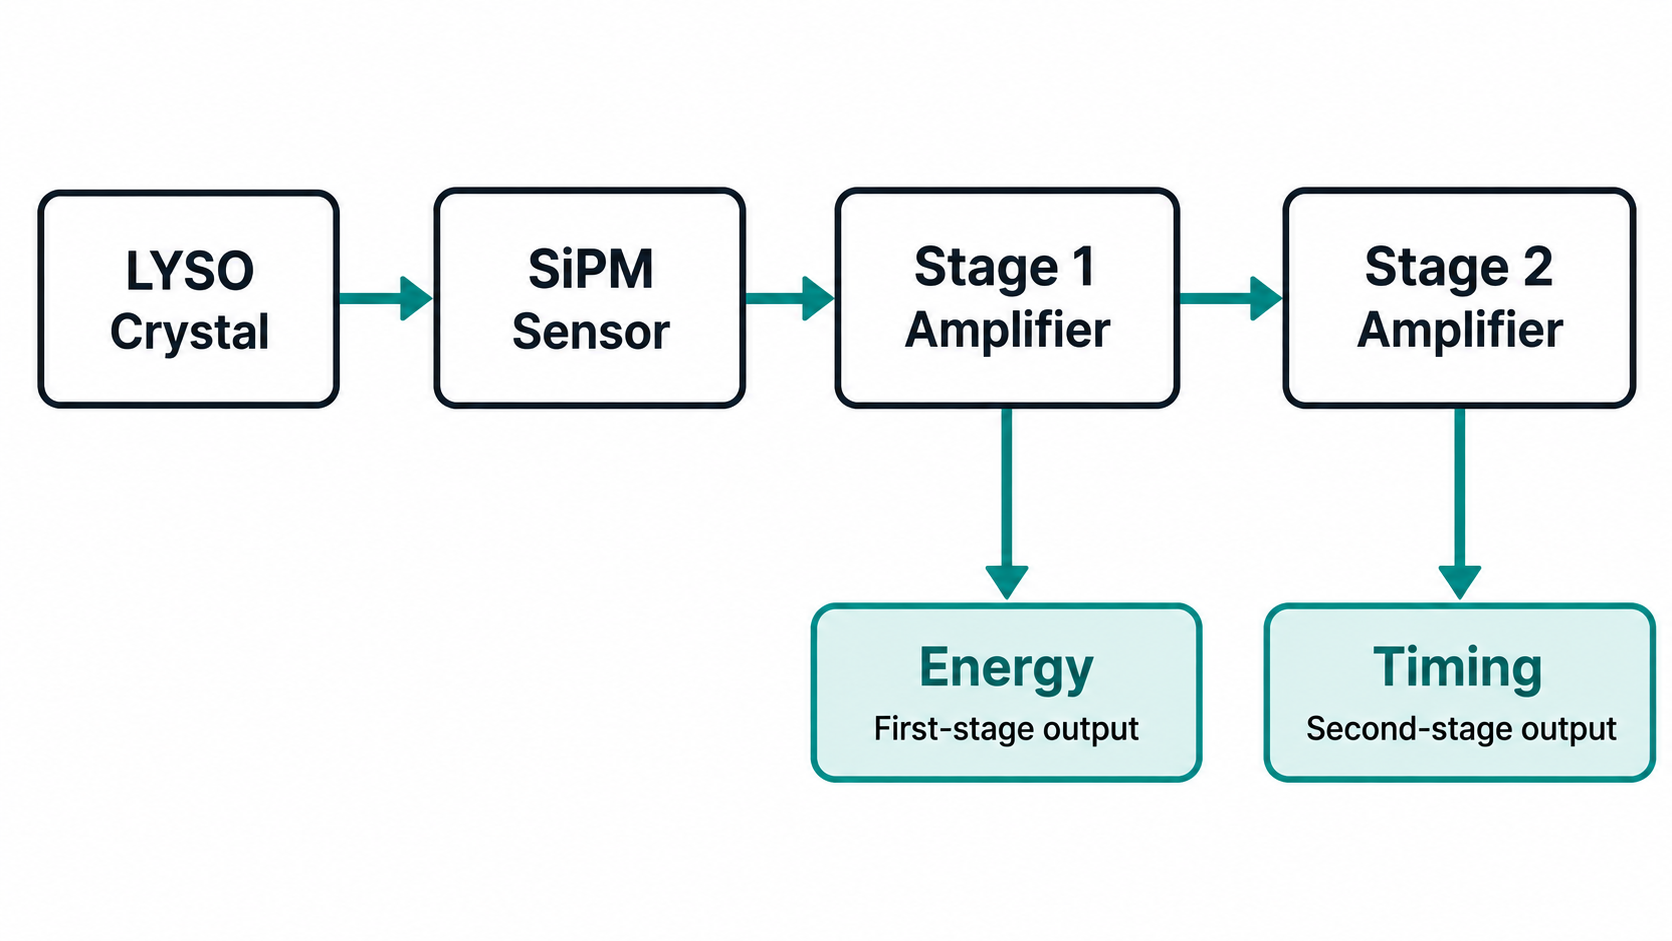
\includegraphics[width=\columnwidth]{figures/Amplifier_schema.png}
\caption{Two-stage analog readout chain used for each detector.
The first-stage (energy) and second-stage (timing) outputs
are acquired simultaneously from the same SiPM pulse.}
\label{fig:amplification-stages}
\end{figure}

The energy waveform is acquired without amplitude clipping,
allowing its maximum to be used for photopeak event selection.
In contrast, the oscilloscope vertical range for the high-gain
timing waveform is deliberately restricted to emphasize the
rising edge, clipping the pulse peak. This acquisition strategy,
also adopted by Onishi et al.~\cite{onishi2022}, aims to
maximize timing precision. In these measurements, the energy
waveform is cleaner and more stable but exhibits greater
time walk, whereas the timing waveform is more susceptible
to noise and pulse-shape variations.

Each coincidence event contains four simultaneously recorded
waveforms: energy signals from the two detectors on channels
1 and 2, and their corresponding timing signals on channels
3 and 4. The records span $100\,\mathrm{ns}$ at a sampling
rate of $80\,\mathrm{GS\,s}^{-1}$. Both waveform modes share
the same energy-based event selection, while timing corrections
are evaluated independently for each amplification stage
and electronics board.


\subsection{Acquisitions and scientific roles}
The benchmark datasets identify three independent acquisitions at a SiPM bias of
$48\,\mathrm{V}$ for each board: control, train and test sets.
The configured true TOF is zero for these centred-source acquisitions.
Control determines the preprocessing and LED selection rules. The train set provides all
model training and selection data. The test set supplies the final test population.

Raw coincidence examples from event 0 are shown separately for each electronics
board: Figures~\ref{fig:uc-raw-energy} and~\ref{fig:uc-raw-timing} show the UC
energy and timing waveforms, while Figures~\ref{fig:fbk-raw-energy}
and~\ref{fig:fbk-raw-timing} show the corresponding FBK waveforms.
Each figure contains the two detector signals from the same coincidence event,
with a shared time axis in nanoseconds relative to the oscilloscope trigger signal.
The waveforms are displayed before event selection or signal preprocessing;
only the sample amplitudes are clipped to the oscilloscope vertical-scale range.

\begin{figure}[H]
\centering
\IfFileExists{figures/UC_raw_energy_event_0.png}{%
  \includegraphics[width=\columnwidth]{figures/UC_raw_energy_event_0.png}%
}{%
  \fbox{\parbox[c][3cm][c]{0.9\columnwidth}{\centering
    \textit{UC raw energy waveform figure}}}%
}
\caption{UC first-stage (energy) waveforms from coincidence event 0.
\textit{[Placeholder: short image description.]}}
\label{fig:uc-raw-energy}
\end{figure}

\begin{figure}[H]
\centering
\IfFileExists{figures/UC_raw_timing_event_0.png}{%
  \includegraphics[width=\columnwidth]{figures/UC_raw_timing_event_0.png}%
}{%
  \fbox{\parbox[c][3cm][c]{0.9\columnwidth}{\centering
    \textit{UC raw timing waveform figure}}}%
}
\caption{UC second-stage (timing) waveforms from coincidence event 0.
\textit{[Placeholder: short image description.]}}
\label{fig:uc-raw-timing}
\end{figure}

\begin{figure}[H]
\centering
\IfFileExists{figures/FBK_raw_energy_event_0.png}{%
  \includegraphics[width=\columnwidth]{figures/FBK_raw_energy_event_0.png}%
}{%
  \fbox{\parbox[c][3cm][c]{0.9\columnwidth}{\centering
    \textit{FBK raw energy waveform figure}}}%
}
\caption{FBK first-stage (energy) waveforms from coincidence event 0.
\textit{[Placeholder: short image description.]}}
\label{fig:fbk-raw-energy}
\end{figure}

\begin{figure}[H]
\centering
\IfFileExists{figures/FBK_raw_timing_event_0.png}{%
  \includegraphics[width=\columnwidth]{figures/FBK_raw_timing_event_0.png}%
}{%
  \fbox{\parbox[c][3cm][c]{0.9\columnwidth}{\centering
    \textit{FBK raw timing waveform figure}}}%
}
\caption{FBK second-stage (timing) waveforms from coincidence event 0.
\textit{[Placeholder: short image description.]}}
\label{fig:fbk-raw-timing}
\end{figure}

Event counts denote coincidence events, each containing four recorded waveforms, and
refer to the final populations available for each waveform mode and window,
after the complete selection described below. The population can change when the mode or
window changes, because an event must satisfy the applicable timing requirements and provide
the requested waveform interval. Within a fixed board, mode and window, models use the same
prepared train and test populations. Selected-event counts are organized by mode
and window in Tables~\ref{tab:uc-selected-events} and~\ref{tab:fbk-selected-events}.

\begin{table*}[t]
\centering
\small
\begin{tabular}{lllr}
\toprule
Mode & Window [ns] & Population & Selected events \\
\midrule
\multirow[t]{6}{*}{Energy}
 & \multirow[t]{3}{*}{Onishi ($-1.5$ to $2$)}
 & Calibration & 16632 \\
 & & Train & 75941 \\
 & & Test & 76315 \\
\addlinespace[3pt]
\cdashline{2-4}
\addlinespace[3pt]
 & \multirow[t]{3}{*}{Wide ($-2$ to $30$)}
 & Calibration & 16627 \\
 & & Train & 75926 \\
 & & Test & 76294 \\
\addlinespace[3pt]
\hdashline
\addlinespace[3pt]
\multirow[t]{6}{*}{Timing}
 & \multirow[t]{3}{*}{Onishi ($-1.5$ to $2$)}
 & Calibration & 14388 \\
 & & Train & 64878 \\
 & & Test & 64763 \\
\addlinespace[3pt]
\cdashline{2-4}
\addlinespace[3pt]
 & \multirow[t]{3}{*}{Wide ($-2$ to $30$)}
 & Calibration & 14388 \\
 & & Train & 64878 \\
 & & Test & 64763 \\
\bottomrule
\end{tabular}
\caption{UC selected event populations by amplification stage
and waveform window, after event selection, LED coincidence
requirements and window availability.}
\label{tab:uc-selected-events}
\end{table*}


\begin{table*}[t]
\centering
\small
\begin{tabular}{lll S[table-format=5.0]}
\toprule
Mode & Window [ns] & Population & {Selected events} \\
\midrule
\multirow[t]{6}{*}{Energy}
 & \multirow[t]{3}{*}{Onishi ($-1.5$ to $2$)}
 & Control & 15488 \\
 & & Development & 77252 \\
 & & Blind & 80365 \\
\addlinespace[3pt]
\cdashline{2-4}
\addlinespace[3pt]
 & \multirow[t]{3}{*}{Wide ($-2$ to $30$)}
 & Control & 15482 \\
 & & Development & 77227 \\
 & & Blind & 80346 \\
\addlinespace[3pt]
\hdashline
\addlinespace[3pt]
\multirow[t]{6}{*}{Timing}
 & \multirow[t]{3}{*}{Onishi ($-1.5$ to $2$)}
 & Control & 14107 \\
 & & Development & 70385 \\
 & & Blind & 73227 \\
\addlinespace[3pt]
\cdashline{2-4}
\addlinespace[3pt]
 & \multirow[t]{3}{*}{Wide ($-2$ to $30$)}
 & Control & 14107 \\
 & & Development & 70385 \\
 & & Blind & 73227 \\
\bottomrule
\end{tabular}
\caption{FBK selected event populations by waveform mode and
input window, after event selection, LED coincidence requirements
and window availability.}
\label{tab:fbk-selected-events}
\end{table*}


\section{Methods}

\subsection{Event selection and LED calibration}
Only photopeak events are retained, based on the maximum amplitudes of both
first-stage (energy) waveforms. Acceptance intervals are obtained from iterative
Gaussian fits to the photopeaks in the calibration acquisition and applied to
both waveform modes. For timing-mode analysis, time-over-threshold (ToT)
selection additionally rejects short, spurious crossings associated with
noise and signal oscillations. Events with excessive pre-pulse baseline
fluctuations or baseline samples near the acquisition limits are excluded.
All selection criteria are established from calibration data only.

For each mode, a leading-edge discriminator (LED) threshold is chosen on the
calibration acquisition to minimize coincidence timing resolution (CTR),
subject to a minimum fraction of valid coincidences within the prescribed
time range. A fixed channel-pair timing offset is subsequently estimated
from the calibration LED residuals. Both the threshold and offset remain
unchanged in training and testing.

\subsection{Timing-error model and learning target}
The goal is to correct waveform-dependent errors in a conventional LED
measurement, rather than estimate an unconstrained time of flight directly.
For a coincidence event, let
$\Delta t_{\mathrm{LED}}=t_{1,\mathrm{LED}}-t_{2,\mathrm{LED}}$.
We model this measurement as
\begin{equation}
\Delta t_{\mathrm{LED}}
=\tau+C+\delta(s_1,s_2)+\epsilon ,
\label{eq:led-error-model}
\end{equation}
where $\tau$ is the true time of flight and $C$ is the fixed
channel-pair offset. The quantities $s_1$ and $s_2$ denote the local
waveform segments of detectors 1 and 2, respectively. The term
$\delta(s_1,s_2)$ represents the waveform-dependent timing error,
while $\epsilon$ accounts for residual unpredictable variation.
The waveform-dependent component $\delta$ is the quantity we aim to estimate 
and correct using ML.

Writing $\widehat C$ for the fixed offset estimated during
calibration, the supervised target  is
\begin{align}
y &= \Delta t_{\mathrm{LED}}-\tau-\widehat C,
\label{eq:ml-target}
\end{align}

and the corrected time difference is

\begin{align}
\widehat{\Delta t}
&=\Delta t_{\mathrm{LED}}-\widehat C
-h_\theta(s_1,s_2).
\label{eq:corrected-time}
\end{align}



The final residual relative to true TOF is:
\begin{align}
r=\widehat{\Delta t}-\tau=y-h_\theta(s_1,s_2).
\label{eq:residual}
\end{align}

This formulation separates waveform-dependent timing errors, 
which can potentially be corrected, from unpredictable noise. 
The source is positioned centrally between the detectors, 
giving $\tau=0$. 
Any positioning error would introduce a constant offset, 
which can be absorbed into the calibration term without affecting CTR.

Energy and timing waveforms are analyzed separately. Each input waveform
is expressed relative to its own LED crossing and normalized using
fixed channel-specific amplitude limits. This alignment removes
absolute acquisition time from the input.
Two LED-relative windows are considered. The short Onishi-inspired
window extends from $-1.5$ to $+2\,\mathrm{ns}$ and follows the
short rising-edge interval used in previous waveform-based timing
work~\cite{onishi2022}. The wide window extends from $-2$ to
$+30\,\mathrm{ns}$, covering a substantially larger portion of the
available acquisition record. Before constant-sample removal, the two
windows contain 279 and 2559 samples per detector, respectively.
For the clipped timing signals, constant sample positions are removed
using the training population; the resulting input sizes are reported
in Table~\ref{tab:input-windows}. No samples are removed from the
energy waveforms. Events lacking a valid coincidence or the full
requested window are excluded.

\begin{table}[tbp]
\centering
\caption{Waveform windows relative to the LED crossing and number of retained samples after constant-sample removal.}
\label{tab:input-windows}
\begin{tabular}{llcc}
\toprule
Board & Signal & Onishi-inspired & Wide \\
\midrule
UC  & Energy & 279 & 2559 \\
UC  & Timing & 136 & 991 \\
FBK & Energy & 279 & 2559 \\
FBK & Timing & 138 & 1944 \\
\bottomrule
\end{tabular}
\end{table}


\subsection{Detector-shared and direct corrections}

Previous waveform-based timing studies have primarily used direct
estimators, which predict the timing correction from the pair of
detector waveforms~\cite{berg2018,onishi2022}. These models can
learn detector-specific relationships without imposing constraints
on how the correction changes when the detector inputs are exchanged.

While effective in a two-detector setup, training a separate model
for every detector pair would be difficult to scale to a complete
PET system. This motivates a detector-shared formulation, in which
the correction is expressed as the difference between two evaluations
of the same function:
\begin{equation}
h_\theta(s_1,s_2)=g_\theta(s_1)-g_\theta(s_2).
\label{eq:shared}
\end{equation}
The shared function $g_\theta$ estimates a waveform-dependent
timing contribution for each detector independently. This formulation
enforces detector-exchange antisymmetry: swapping the inputs
reverses the correction sign, while identical inputs yield zero
correction. It also offers a potentially more scalable approach, 
since the same model can be applied to different physical instances 
of the same detector type, without requiring parameters specific 
to each detector pair.

To characterize how the choice of estimator affects waveform-based timing
correction, we consider model families with different inductive biases.
Linear ridge regression provides a simple and stable baseline. 
MiniRocket provides an efficient time-series-specific representation. 
MLPs provide a general nonlinear estimator
without explicitly exploiting temporal locality, whereas CNNs incorporate
local waveform structure and are included both as a standard time-series
architecture and because of their successful use in previous waveform-based
timing studies~\cite{onishi2022,loignon2025}. Locally connected networks
retain the local receptive-field structure of CNNs while allowing the learned
response to depend on absolute temporal position, which is relevant here
because the waveforms are aligned to the LED crossing.
Table~\ref{tab:model-inventory} summarizes the resulting estimators, while
implementation details are provided in the appendix.

\subsection{Model comparison and training protocol}
The independent calibration, training and test acquisitions serve distinct
roles, as summarized in Figure~\ref{fig:workflow}. Calibration fixes event
selection, LED thresholds and timing offsets. Model fitting and selection
use only the training set; the test set is reserved for
final evaluation.

The models are trained to predict the LED timing error using
a standard regression objective, the mean squared error (MSE):
\begin{equation}
\mathrm{MSE}=\frac{1}{N}\sum_{i=1}^{N}
\left[y_i-h_\theta(s_{1,i},s_{2,i})\right]^2.
\label{eq:training-mse}
\end{equation}
Model selection is performed through three-fold cross-validation
on the training acquisition, using mean validation CTR as the
primary performance criterion. The selected model is then
refitted on the full training dataset. The independent test
acquisition is subsequently used to compare the observed performance
of the tested estimators. References in the Results section to the
lowest test CTR therefore identify the best observed result within
that specific comparison, rather than a general model ranking.
Model-specific training procedures and exceptions are detailed in
Appendix~\ref{app:spaces}.


\subsection{Timing performance and independent evaluation}
All configurations are evaluated against LED on the same selected
test events. CTR is defined as the full width at half maximum
(FWHM) of the timing-residual distribution and computed using
histogram-based method F1 of Rainio et al.~\cite{rainio2025}.
Identical histogram settings are used for LED and corrected
residuals within each mode. The fixed bin widths are
$10\,\mathrm{ps}$ for energy and $5\,\mathrm{ps}$ for timing.

Root mean squared error (RMSE) relative to true TOF complements
CTR because it captures both residual dispersion and systematic
bias. In particular,
$\mathrm{MSE}=\operatorname{Var}(r)+[\mathbb{E}(r)]^2$;
a reduction in RMSE need not imply a comparable narrowing
of the central timing peak. Both metrics are therefore needed
to characterize the effects of calibration and waveform-based
correction.

Fixed preprocessing and the fitted model are applied to the
independent test acquisition. Test-event bootstrap resampling
provides uncertainties on CTR and RMSE without retraining;
these estimates are conditional on the selected fitted model.
Within-board comparisons use matched test events and joint
resampling to assess paired model differences.

\subsection{Temporal sensitivity analysis}
To investigate which parts of each waveform influence the
correction, temporal occlusion is applied to the trained models
on test events. Short groups of samples are replaced by
interpolation from neighboring samples, and their importance
is quantified by the average absolute change in predicted
correction. Shared estimators are perturbed synchronously in
both detector inputs, while direct estimators are perturbed
one input at a time.

The resulting profiles reveal whether predictions depend
primarily on the rising edge or also on later waveform
characteristics, and allow comparisons across windows and
amplification stages.

\begin{table*}[t]
\centering
\small
\begin{tabularx}{\textwidth}{@{}p{0.12\textwidth}p{0.08\textwidth}p{0.24\textwidth}X@{}}
\toprule
Formulation & Code & Estimator & Correction structure \\
\midrule
Direct & D-LIN & Linear ridge & Joint linear regression on concatenated waveforms. \\
Direct & D-MLP & Dense MLP & Joint nonlinear regression on concatenated waveforms. \\
Direct & D-CNN & Independent CNN & Separate detector-specific CNN scorers; output difference. \\
Direct & D-ONI & Onishi-inspired CNN & Paired waveforms fused by convolution for joint regression. \\
Direct & D-MR & MiniRocket + ridge & Multivariate features of the waveform pair; ridge regression. \\
\addlinespace[3pt]
Shared & S-LIN & Linear ridge & Linear regression on the difference of waveform samples. \\
Shared & S-MLP & Dense MLP & Common nonlinear detector scorer; output difference. \\
Shared & S-LCM & Locally connected MLP & Common position-specific local scorer; bounded output difference. \\
Shared & S-CNN & Temporal CNN & Common convolutional detector scorer; output difference. \\
Shared & S-MR & MiniRocket + ridge & Common waveform feature transform; feature difference and ridge regression. \\
\bottomrule
\end{tabularx}
\caption{Waveform-based timing estimators implemented in the benchmark. Model
codes are used throughout the results tables. Direct estimators do not enforce
detector-exchange antisymmetry; shared estimators use a common detector-level
function or feature transform to enforce it.}
\label{tab:model-inventory}
\end{table*}

\begin{figure*}[t]
\centering
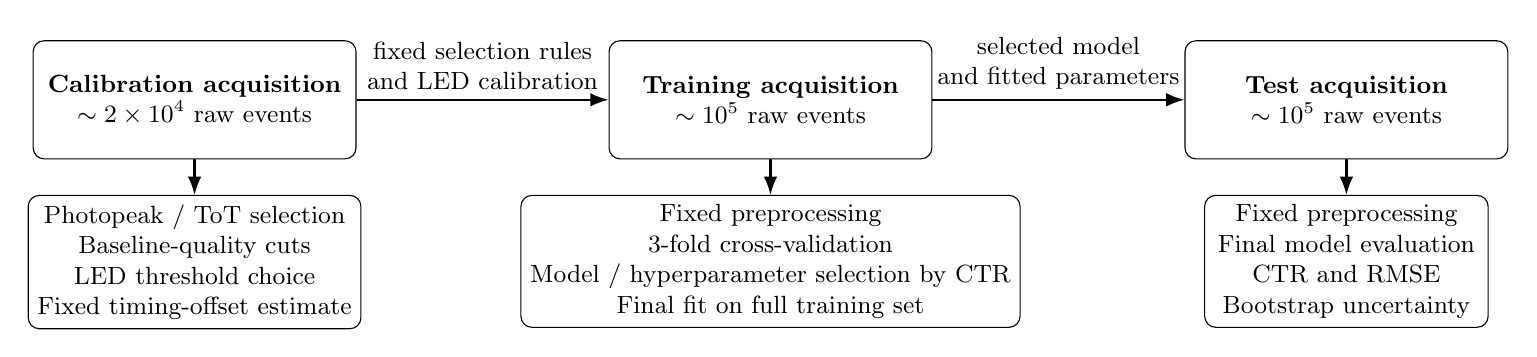
\begin{tikzpicture}[
    node distance=1.8cm and 1.8cm,
    >=Latex,
    box/.style={
        draw,
        rounded corners,
        align=center,
        minimum width=4.1cm,
        minimum height=1.5cm,
        font=\small
    },
    smallbox/.style={
        draw,
        rounded corners,
        align=center,
        minimum width=3.6cm,
        minimum height=1.1cm,
        font=\small
    },
    arrow/.style={->, thick}
]

\node[box] (cal) {
    \textbf{Calibration acquisition}\\
    $\sim 2\times 10^4$ raw events
};

\node[smallbox, below=0.45cm of cal] (caluse) {
    Photopeak / ToT selection\\
    Baseline-quality cuts\\
    LED threshold choice\\
    Fixed timing-offset estimate
};

\node[box, right=3.2cm of cal] (train) {
    \textbf{Training acquisition}\\
    $\sim 10^5$ raw events
};

\node[smallbox, below=0.45cm of train] (trainuse) {
    Fixed preprocessing\\
    3-fold cross-validation\\
    Model / hyperparameter selection by CTR\\
    Final fit on full training set
};

\node[box, right=3.2cm of train] (test) {
    \textbf{Test acquisition}\\
    $\sim 10^5$ raw events
};

\node[smallbox, below=0.45cm of test] (testuse) {
    Fixed preprocessing\\
    Final model evaluation\\
    CTR and RMSE\\
    Bootstrap uncertainty
};

\draw[arrow] (cal.east) -- node[above, font=\small, align=center] {fixed selection rules\\and LED calibration} (train.west);
\draw[arrow] (train.east) -- node[above, font=\small, align=center] {selected model\\and fitted parameters} (test.west);

\draw[arrow] (cal) -- (caluse);
\draw[arrow] (train) -- (trainuse);
\draw[arrow] (test) -- (testuse);

\end{tikzpicture}
\caption{Schematic overview of the experimental protocol. The calibration acquisition is used to determine fixed event-selection and LED-calibration criteria. Model selection and fitting are performed on the independent training acquisition. Final performance is assessed on the independent test acquisition.}
\label{fig:workflow}
\end{figure*}



\section{Results}
\label{sec:results-tables}
% Independent-test metrics are reported as CTR and RMSE; plots of all CTR
% comparisons appear in Appendix~\ref{app:ctr-plots}.

Differences of only a few picoseconds among the leading estimators are
reported descriptively and are not interpreted as evidence of a generally
superior architecture. Such differences are comparable to the scale of the
reported uncertainties and may depend on the detector and acquisition
configuration. The discussion therefore focuses on larger and recurring
trends across boards, waveform modes, and input windows.

\subsection{University of Chicago board}

\subsubsection{Energy waveforms}
Energy-waveform corrections reduce the test CTR from the LED reference of
approximately $142\,\mathrm{ps}$ to $110.5\,\mathrm{ps}$ with the short
Onishi-inspired window and $105.3\,\mathrm{ps}$ with the wide window
(Tables~\ref{tab:uc-energy-onishi} and~\ref{tab:uc-energy-wide};
Figures~\ref{fig:uc-energy-onishi-ctr} and~\ref{fig:uc-energy-wide-ctr}).
The Onishi-inspired paired CNN gives the lowest observed test CTR for the
short window, while several shared and direct estimators fall within the
same few-picosecond performance range. With the wide window, direct
linear ridge gives the lowest observed CTR, again with several other
estimators nearby. The relevant trend is the improvement obtained by
extending the waveform window rather than the exact ordering of the
leading models. Most models show lower CTR and RMSE with the longer
window, although the magnitude of the improvement differs by architecture.
The independent temporal CNN is a notable exception to the relatively
close model agreement in the short-window comparison and remains among
the weaker results in the wide-window setting.

% Generated by report/generate_results_tables.py; do not edit manually.
% LED bootstrap uncertainty source model: antisymmetric_mlp
\begin{table*}[tbp]
\centering
\small
\begin{tabularx}{\textwidth}{@{}lXccc@{}}
\toprule
Code & Estimator & Validation CTR [ps] & Test CTR [ps] & Test RMSE [ps] \\
\midrule
LED & Leading-edge reference & --- & $142.20 \pm 1.66$ & $68.08 \pm 1.11$ \\
\midrule
D-ONI & Onishi-inspired paired CNN & $111.03 \pm 1.27$ & $110.50 \pm 1.23$ & $56.96 \pm 1.32$ \\
S-MR & Shared MiniRocket + ridge & $111.83 \pm 3.33$ & $111.96 \pm 1.21$ & $57.38 \pm 1.33$ \\
S-CNN & Shared temporal CNN & $113.07 \pm 1.58$ & $112.46 \pm 1.20$ & $57.59 \pm 1.32$ \\
D-MR & Direct MiniRocket + ridge & $111.35 \pm 3.35$ & $112.50 \pm 1.41$ & $57.62 \pm 1.34$ \\
S-LIN & Shared linear ridge & n/a & $112.51 \pm 1.24$ & $58.23 \pm 1.33$ \\
S-LCM & Shared locally connected MLP & $112.91 \pm 2.81$ & $112.57 \pm 1.19$ & $57.96 \pm 1.30$ \\
D-LIN & Direct linear ridge & n/a & $112.67 \pm 1.14$ & $57.56 \pm 1.29$ \\
S-MLP & Shared dense MLP & $112.75 \pm 1.45$ & $113.19 \pm 1.28$ & $58.42 \pm 1.27$ \\
D-MLP & Direct dense MLP & $112.94 \pm 1.04$ & $113.60 \pm 1.19$ & $58.05 \pm 1.30$ \\
D-CNN & Independent temporal CNN & $112.80 \pm 1.30$ & $125.16 \pm 1.44$ & $63.08 \pm 1.21$ \\
\bottomrule
\end{tabularx}
\caption{UC board, energy waveforms, onishi window. Validation CTR is the mean $\pm$ standard deviation across held-out CV folds. Test CTR and RMSE are shown with test-event bootstrap standard deviations. LED has no validation score; linear ridge uses internal MSE-based CV, not outer CTR-based validation. Estimators are ordered by test CTR.}
\label{tab:uc-energy-onishi}
\end{table*}

% Generated by report/generate_results_tables.py; do not edit manually.
% LED bootstrap uncertainty source model: antisymmetric_mlp
\begin{table*}[tbp]
\centering
\small
\begin{tabularx}{\textwidth}{@{}lXccc@{}}
\toprule
Code & Estimator & Validation CTR [ps] & Test CTR [ps] & Test RMSE [ps] \\
\midrule
LED & Leading-edge reference & --- & $142.19 \pm 1.69$ & $68.03 \pm 1.13$ \\
\midrule
D-LIN & Direct linear ridge & n/a & $105.32 \pm 1.09$ & $54.82 \pm 1.37$ \\
D-ONI & Onishi-inspired paired CNN & $107.34 \pm 2.87$ & $107.32 \pm 1.23$ & $55.66 \pm 1.39$ \\
S-LIN & Shared linear ridge & n/a & $107.37 \pm 1.31$ & $55.44 \pm 1.32$ \\
S-LCM & Shared locally connected MLP & $107.76 \pm 1.01$ & $107.54 \pm 1.27$ & $55.54 \pm 1.28$ \\
S-CNN & Shared temporal CNN & $105.20 \pm 0.47$ & $107.98 \pm 1.19$ & $55.62 \pm 1.30$ \\
S-MLP & Shared dense MLP & $106.34 \pm 1.88$ & $108.18 \pm 1.25$ & $55.61 \pm 1.36$ \\
D-MR & Direct MiniRocket + ridge & $108.45 \pm 1.92$ & $108.99 \pm 1.17$ & $56.48 \pm 1.33$ \\
S-MR & Shared MiniRocket + ridge & $109.77 \pm 0.28$ & $109.02 \pm 1.45$ & $56.42 \pm 1.36$ \\
D-MLP & Direct dense MLP & $130.98 \pm 3.93$ & $115.61 \pm 1.26$ & $58.68 \pm 1.27$ \\
D-CNN & Independent temporal CNN & $128.03 \pm 9.32$ & $123.52 \pm 1.64$ & $62.44 \pm 1.24$ \\
\bottomrule
\end{tabularx}
\caption{UC board, energy waveforms, wide window. Validation CTR is the mean $\pm$ standard deviation across held-out CV folds. Test CTR and RMSE are shown with test-event bootstrap standard deviations. LED has no validation score; linear ridge uses internal MSE-based CV, not outer CTR-based validation. Estimators are ordered by test CTR.}
\label{tab:uc-energy-wide}
\end{table*}


\subsubsection{Timing waveforms}
The timing-waveform LED reference is approximately $57.1\,\mathrm{ps}$.
With the short window, most estimators remain close to this reference,
and the lowest observed test CTR is $56.3\,\mathrm{ps}$. With the wide
window, the minimum decreases to $52.9\,\mathrm{ps}$, and several linear,
MiniRocket-based and shared estimators lie between approximately
$53$ and $54\,\mathrm{ps}$
(Tables~\ref{tab:uc-timing-onishi} and~\ref{tab:uc-timing-wide};
Figures~\ref{fig:uc-timing-onishi-ctr} and~\ref{fig:uc-timing-wide-ctr}).
Thus, extending the timing input produces a clearer improvement in CTR
than the small short-window corrections. The short-window direct
MiniRocket result is an outlier, with a test CTR exceeding the LED
reference. RMSE changes are generally smaller than the corresponding
CTR changes.

% Generated by report/generate_results_tables.py; do not edit manually.
% LED bootstrap uncertainty source model: antisymmetric_mlp
\begin{table*}[tbp]
\centering
\small
\begin{tabularx}{\textwidth}{@{}lXccc@{}}
\toprule
Code & Estimator & Validation CTR [ps] & Test CTR [ps] & Test RMSE [ps] \\
\midrule
LED & Leading-edge reference & --- & $57.10 \pm 0.65$ & $36.58 \pm 1.71$ \\
\midrule
S-MLP & Shared dense MLP & $57.30 \pm 1.53$ & $56.25 \pm 0.74$ & $36.43 \pm 1.71$ \\
S-LIN & Shared linear ridge & n/a & $56.43 \pm 0.63$ & $36.25 \pm 1.64$ \\
D-ONI & Onishi-inspired paired CNN & $56.88 \pm 0.33$ & $56.55 \pm 0.69$ & $36.70 \pm 1.66$ \\
S-LCM & Shared locally connected MLP & $56.96 \pm 0.89$ & $56.60 \pm 0.70$ & $36.41 \pm 1.70$ \\
D-LIN & Direct linear ridge & n/a & $56.69 \pm 0.58$ & $36.24 \pm 1.68$ \\
D-CNN & Independent temporal CNN & $57.56 \pm 0.43$ & $56.71 \pm 0.69$ & $36.58 \pm 1.73$ \\
S-CNN & Shared temporal CNN & $57.50 \pm 1.05$ & $56.78 \pm 0.64$ & $36.34 \pm 1.68$ \\
D-MLP & Direct dense MLP & $57.46 \pm 0.42$ & $56.90 \pm 0.66$ & $36.58 \pm 1.74$ \\
S-MR & Shared MiniRocket + ridge & $57.13 \pm 0.28$ & $57.27 \pm 0.61$ & $35.29 \pm 1.24$ \\
D-MR & Direct MiniRocket + ridge & $68.82 \pm 2.75$ & $64.89 \pm 0.74$ & $38.03 \pm 1.16$ \\
\bottomrule
\end{tabularx}
\caption{UC board, timing waveforms, onishi window. Validation CTR is the mean $\pm$ standard deviation across held-out CV folds. Test CTR and RMSE are shown with test-event bootstrap standard deviations. LED has no validation score; linear ridge uses internal MSE-based CV, not outer CTR-based validation. Estimators are ordered by test CTR.}
\label{tab:uc-timing-onishi}
\end{table*}

% Generated by report/generate_results_tables.py; do not edit manually.
% LED bootstrap uncertainty source model: antisymmetric_mlp
\begin{table*}[tbp]
\centering
\small
\begin{tabularx}{\textwidth}{@{}lXccc@{}}
\toprule
Code & Estimator & Validation CTR [ps] & Test CTR [ps] & Test RMSE [ps] \\
\midrule
LED & Leading-edge reference & --- & $57.10 \pm 0.65$ & $36.58 \pm 1.71$ \\
\midrule
D-MR & Direct MiniRocket + ridge & $54.09 \pm 0.34$ & $52.91 \pm 0.78$ & $35.61 \pm 1.70$ \\
S-MR & Shared MiniRocket + ridge & $54.88 \pm 1.27$ & $53.51 \pm 0.77$ & $35.39 \pm 1.58$ \\
D-LIN & Direct linear ridge & n/a & $53.51 \pm 0.65$ & $35.39 \pm 1.72$ \\
S-LIN & Shared linear ridge & n/a & $53.66 \pm 0.66$ & $35.46 \pm 1.67$ \\
S-CNN & Shared temporal CNN & $54.83 \pm 0.80$ & $54.55 \pm 0.61$ & $35.64 \pm 1.71$ \\
D-MLP & Direct dense MLP & $55.12 \pm 1.28$ & $54.89 \pm 0.59$ & $35.92 \pm 1.77$ \\
D-ONI & Onishi-inspired paired CNN & $54.97 \pm 0.41$ & $55.01 \pm 0.64$ & $35.75 \pm 1.70$ \\
S-LCM & Shared locally connected MLP & $54.31 \pm 0.58$ & $55.44 \pm 0.51$ & $35.96 \pm 1.72$ \\
S-MLP & Shared dense MLP & $54.88 \pm 1.16$ & $55.77 \pm 0.58$ & $36.00 \pm 1.73$ \\
D-CNN & Independent temporal CNN & $57.63 \pm 1.61$ & $56.86 \pm 0.69$ & $36.58 \pm 1.73$ \\
\bottomrule
\end{tabularx}
\caption{UC board, timing waveforms, wide window. Validation CTR is the mean $\pm$ standard deviation across held-out CV folds. Test CTR and RMSE are shown with test-event bootstrap standard deviations. LED has no validation score; linear ridge uses internal MSE-based CV, not outer CTR-based validation. Estimators are ordered by test CTR.}
\label{tab:uc-timing-wide}
\end{table*}


\subsubsection{Temporal sensitivity: wide window}
The temporal-occlusion maps for the lowest-test-CTR wide-window
estimators are shown in Figures~\ref{fig:uc-energy-wide-xai}
and~\ref{fig:uc-timing-wide-xai}. For energy waveforms, the
largest sensitivity is concentrated around LED crossing and the early
rising edge, with weaker sensitivity over the later waveform. In
timing mode, sensitivity is also concentrated near the crossing and
the end of the clipped portion, while a smaller response appears
around the late feature at approximately $21$--$22\,\mathrm{ns}$.
The latter is visible in both detector traces, but its importance
is much lower than that of the early regions.

\begin{figure}[tbp]
\centering
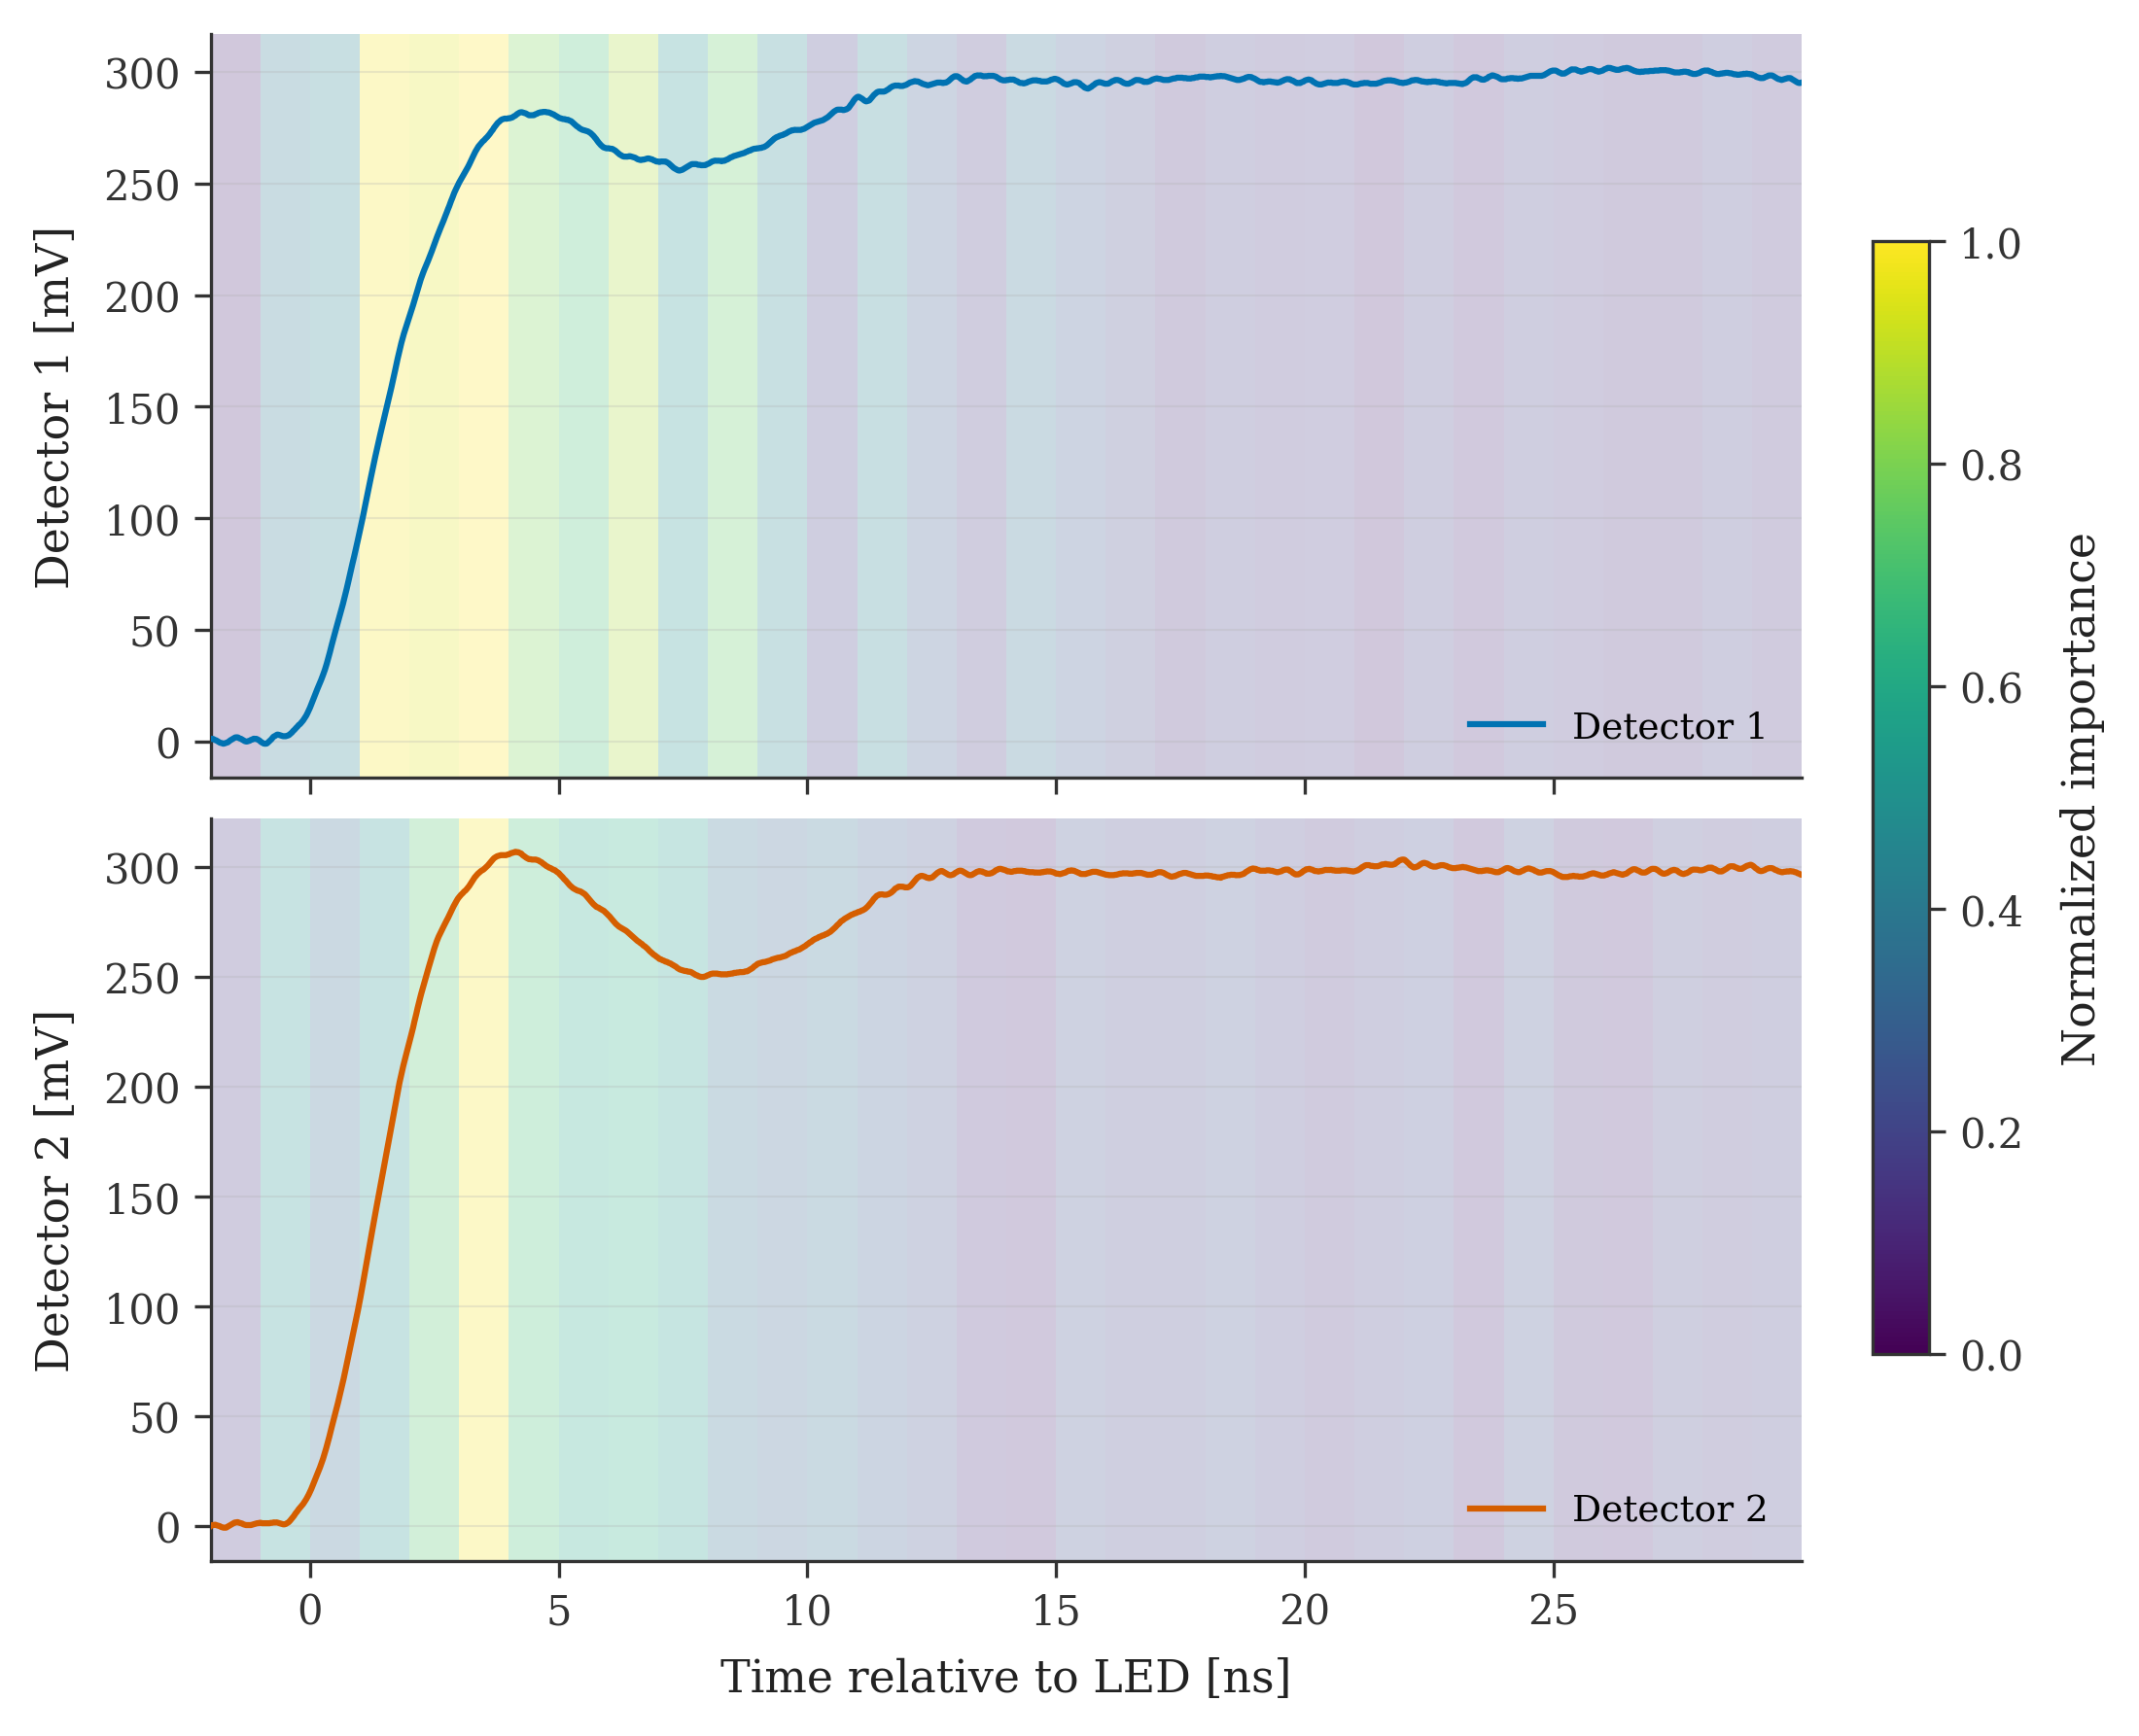
\includegraphics[width=\columnwidth]{figures/xai/energy_UC.png}
\caption{UC energy waveforms, wide window: temporal occlusion sensitivity
of the estimator with the lowest observed test CTR (direct linear ridge), shown against the
two detector waveforms. Colors indicate normalized sensitivity to local
occlusion, not causal attribution.}
\label{fig:uc-energy-wide-xai}
\end{figure}

\begin{figure}[tbp]
\centering
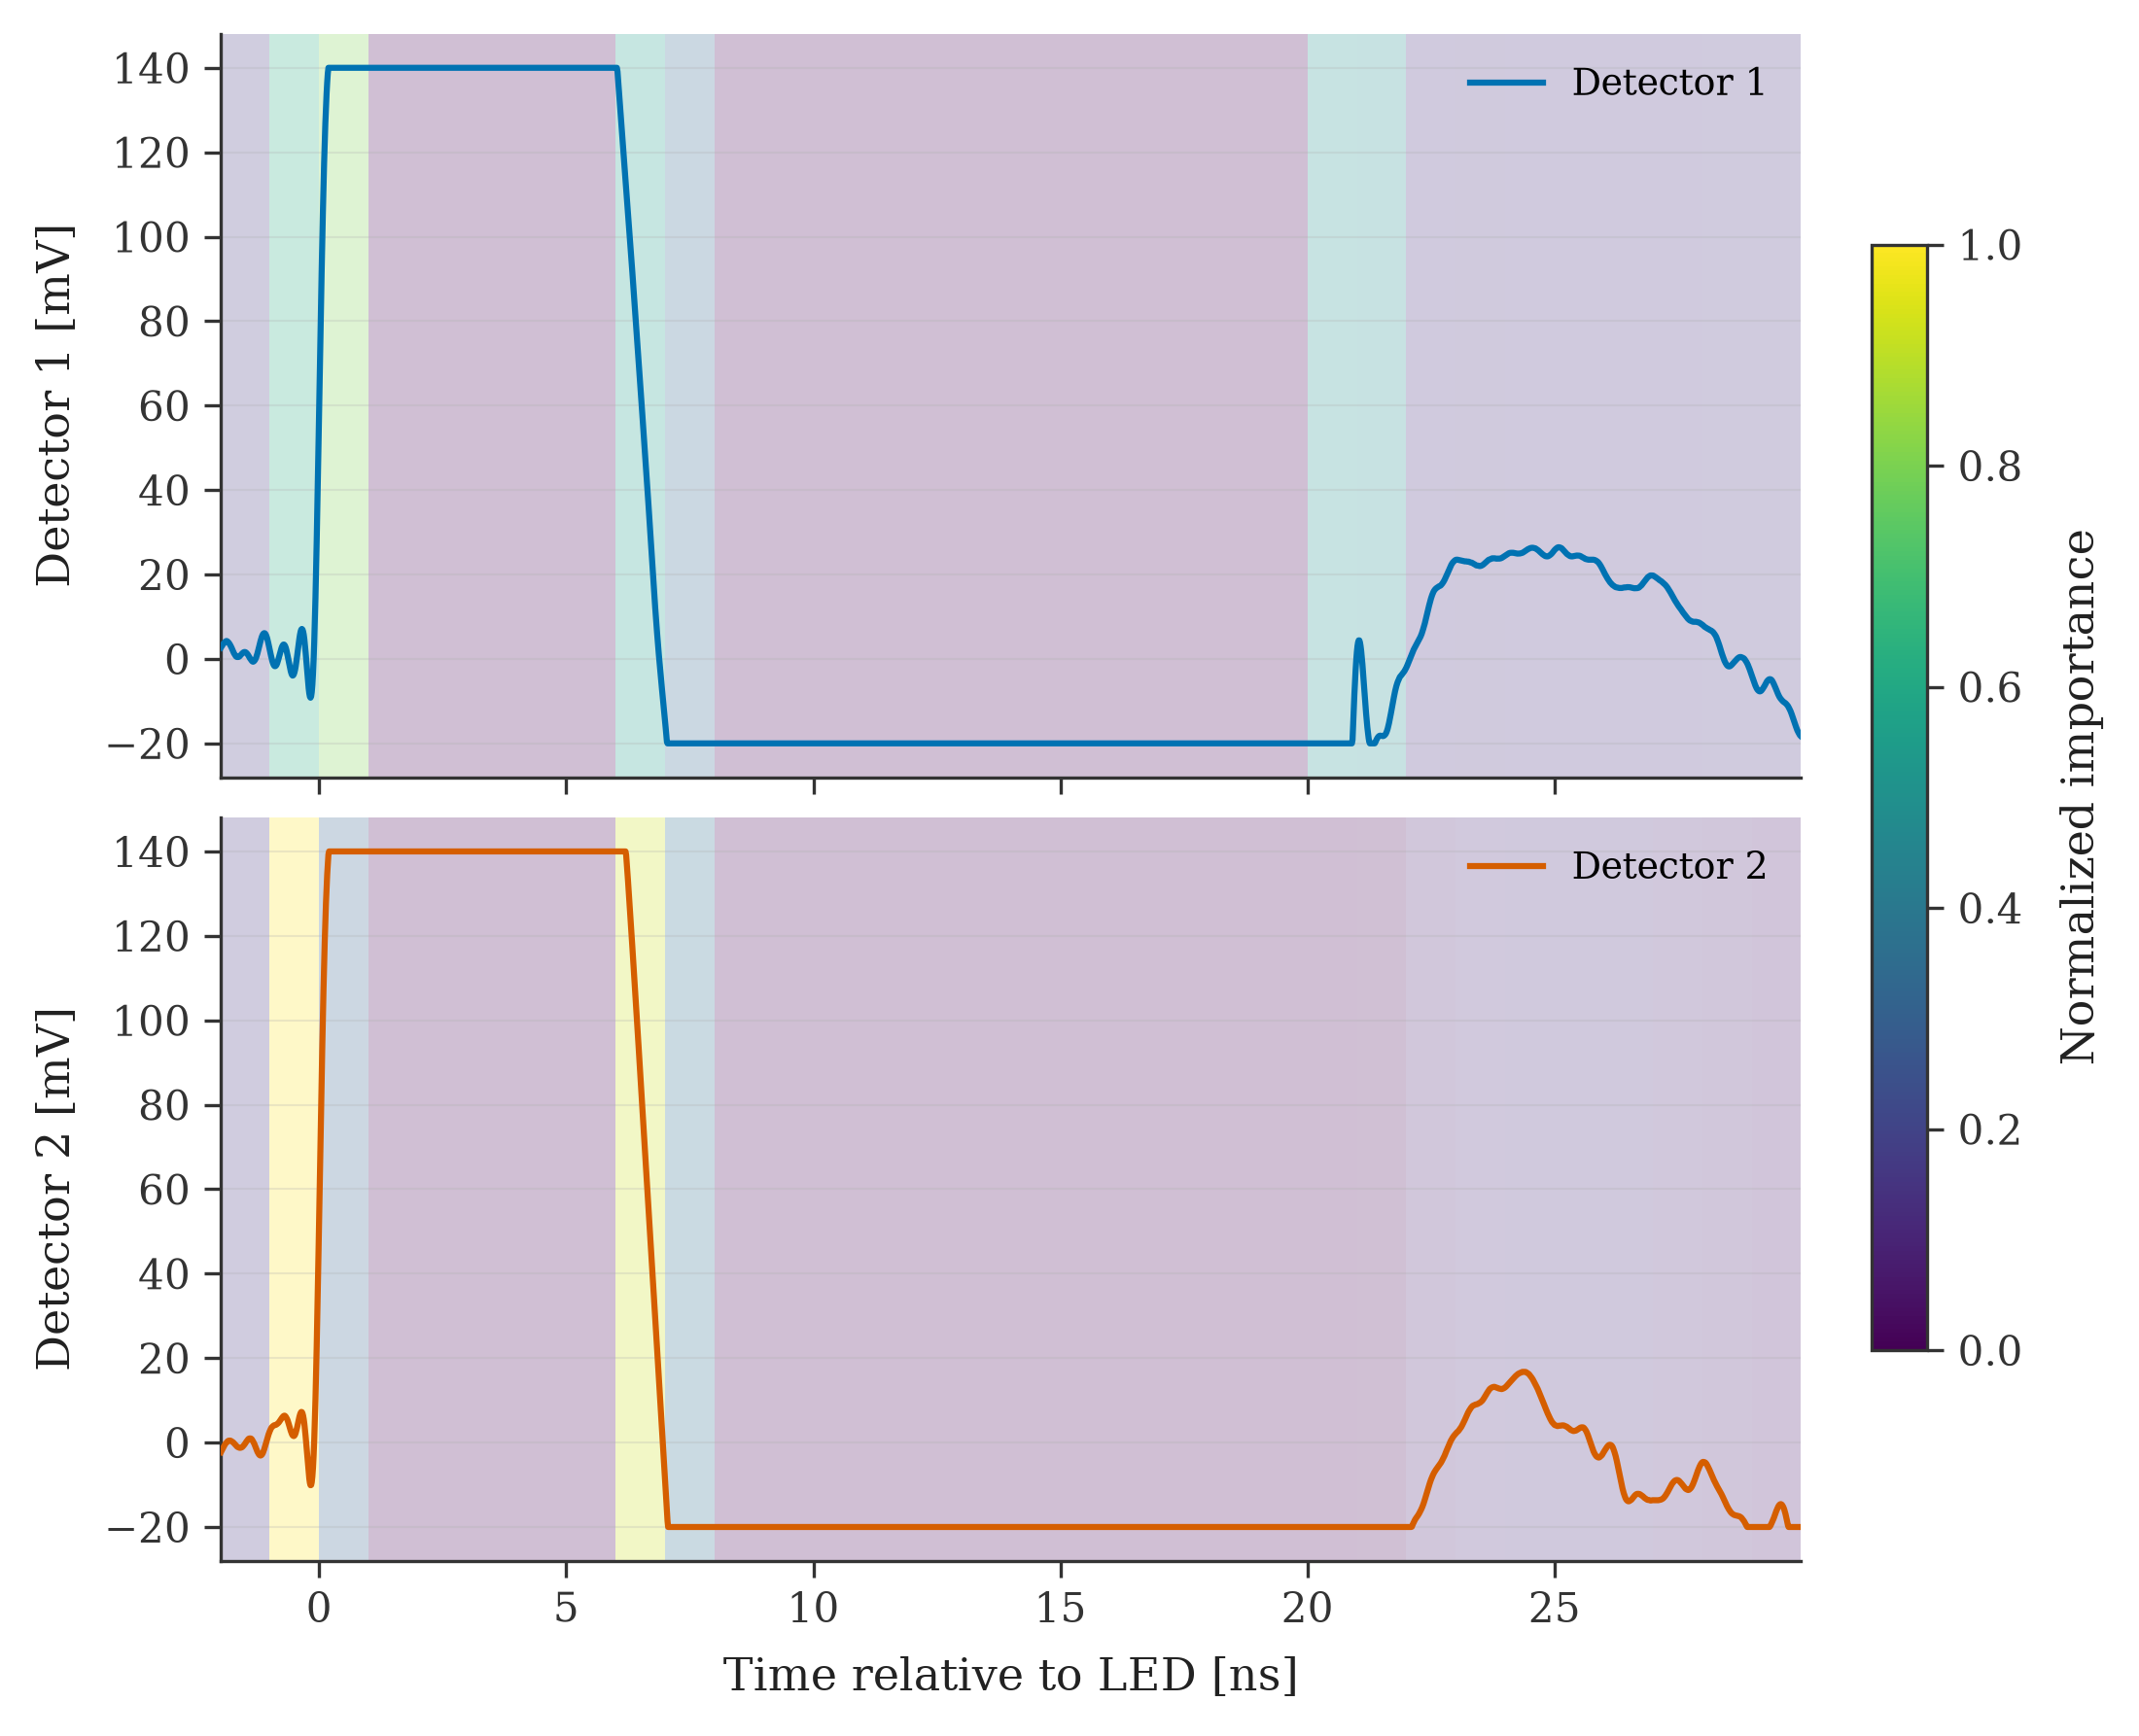
\includegraphics[width=\columnwidth]{figures/xai/timing_UC.png}
\caption{UC timing waveforms, wide window: temporal occlusion sensitivity
of the estimator with the lowest observed test CTR (direct MiniRocket), shown against the
two detector waveforms.}
\label{fig:uc-timing-wide-xai}
\end{figure}

\subsection{Fondazione Bruno Kessler board}

\subsubsection{Energy waveforms}
For FBK energy waveforms, the LED reference is approximately
$147.3\,\mathrm{ps}$. The lowest observed short-window CTR is
$115.4\,\mathrm{ps}$, with linear and nonlinear estimators occupying
a similar performance range
(Table~\ref{tab:fbk-energy-onishi};
Figure~\ref{fig:fbk-energy-onishi-ctr}).
The wide-window minimum is $111.0\,\mathrm{ps}$, obtained with
direct MiniRocket, while several other estimators remain around
$114$--$116\,\mathrm{ps}$
(Table~\ref{tab:fbk-energy-wide};
Figure~\ref{fig:fbk-energy-wide-ctr}).
The shared temporal CNN is a marked wide-window outlier: despite a
validation CTR of approximately $115\,\mathrm{ps}$, the final refit
provides essentially no improvement over LED on the independent test
set. Neural-network optimization is non-convex and stochastic, so
different weight initializations, minibatch sequences, or changes in
the fitting population can lead the same architecture and
hyperparameters to different fitted solutions. The observed discrepancy
is therefore consistent with an unstable final optimization, although
the present analysis does not isolate its specific cause. As with UC,
the strongest wide-window results improve over the short-window minimum,
but individual architectures do not all benefit equally.

% Generated by report/generate_results_tables.py; do not edit manually.
% LED bootstrap uncertainty source model: antisymmetric_mlp
\begin{table}[tbp]
\centering
\scriptsize
\resizebox{\columnwidth}{!}{%
\begin{tabular}{@{}lccc@{}}
\toprule
Model & CV CTR [ps] & Test CTR [ps] & Test RMSE [ps] \\
\midrule
LED & --- & $147.3 \pm 1.8$ & $70.9 \pm 1.0$ \\
\midrule
D-ONI & $114.9 \pm 1.5$ & $115.4 \pm 1.2$ & $60.6 \pm 1.2$ \\
S-LIN & n/a & $115.9 \pm 1.3$ & $62.8 \pm 1.2$ \\
D-LIN & n/a & $116.2 \pm 1.5$ & $61.4 \pm 1.2$ \\
D-MR & $115.9 \pm 2.3$ & $116.4 \pm 1.2$ & $60.8 \pm 1.2$ \\
S-LCM & $117.3 \pm 2.4$ & $116.5 \pm 1.4$ & $62.0 \pm 1.0$ \\
S-CNN & $116.9 \pm 0.1$ & $116.7 \pm 1.4$ & $61.8 \pm 1.1$ \\
D-MLP & $118.6 \pm 1.7$ & $117.7 \pm 1.2$ & $61.5 \pm 1.1$ \\
D-CNN & $123.9 \pm 4.5$ & $117.7 \pm 1.2$ & $61.2 \pm 1.2$ \\
S-MLP & $116.9 \pm 1.9$ & $119.0 \pm 1.4$ & $62.8 \pm 1.2$ \\
S-MR & $116.8 \pm 0.8$ & $120.4 \pm 1.1$ & $61.5 \pm 1.1$ \\
\bottomrule
\end{tabular}%
}
\caption{FBK energy onishi: validation CTR (mean $\pm$ fold SD), independent-test CTR and RMSE (estimate $\pm$ bootstrap SD). Models are ranked by unrounded test CTR; codes are defined in Table~\ref{tab:model-inventory}. LED has no outer CV; ridge uses internal LOOCV.}
\label{tab:fbk-energy-onishi}
\end{table}

% Generated by report/generate_results_tables.py; do not edit manually.
% LED bootstrap uncertainty source model: antisymmetric_mlp
\begin{table*}[tbp]
\centering
\small
\begin{tabularx}{\textwidth}{@{}lXccc@{}}
\toprule
Code & Estimator & Validation CTR [ps] & Test CTR [ps] & Test RMSE [ps] \\
\midrule
LED & Leading-edge reference & --- & $147.30 \pm 1.62$ & $70.93 \pm 1.06$ \\
\midrule
D-MR & Direct MiniRocket + ridge & $111.90 \pm 0.24$ & $111.02 \pm 1.16$ & $58.57 \pm 0.97$ \\
D-LIN & Direct linear ridge & n/a & $114.38 \pm 1.08$ & $59.87 \pm 1.26$ \\
S-LCM & Shared locally connected MLP & $114.72 \pm 0.74$ & $114.94 \pm 1.21$ & $60.08 \pm 1.27$ \\
D-ONI & Onishi-inspired paired CNN & $114.13 \pm 0.93$ & $115.33 \pm 1.36$ & $59.35 \pm 1.07$ \\
S-LIN & Shared linear ridge & n/a & $115.87 \pm 1.17$ & $60.18 \pm 1.32$ \\
S-MLP & Shared dense MLP & $115.31 \pm 0.81$ & $115.87 \pm 1.43$ & $60.25 \pm 1.21$ \\
D-MLP & Direct dense MLP & $119.57 \pm 2.44$ & $116.92 \pm 1.29$ & $60.91 \pm 1.05$ \\
S-MR & Shared MiniRocket + ridge & $117.04 \pm 1.62$ & $117.91 \pm 1.42$ & $59.63 \pm 1.13$ \\
D-CNN & Independent temporal CNN & $131.62 \pm 3.42$ & $130.63 \pm 1.17$ & $65.19 \pm 1.13$ \\
S-CNN & Shared temporal CNN & $115.05 \pm 0.22$ & $147.30 \pm 1.69$ & $70.93 \pm 1.11$ \\
\bottomrule
\end{tabularx}
\caption{FBK board, energy waveforms, wide window. Validation CTR is the mean $\pm$ standard deviation across held-out CV folds. Test CTR and RMSE are shown with test-event bootstrap standard deviations. LED has no validation score; linear ridge uses internal MSE-based CV, not outer CTR-based validation. Estimators are ordered by test CTR.}
\label{tab:fbk-energy-wide}
\end{table*}


\subsubsection{Timing waveforms}
In FBK timing mode, the LED reference is about $62.0\,\mathrm{ps}$.
Short-window test CTRs range from approximately $57.7\,\mathrm{ps}$
to values close to LED, whereas the wide-window comparison reaches a
minimum of $54.4\,\mathrm{ps}$
(Tables~\ref{tab:fbk-timing-onishi} and~\ref{tab:fbk-timing-wide};
Figures~\ref{fig:fbk-timing-onishi-ctr} and~\ref{fig:fbk-timing-wide-ctr}).
The leading wide-window results are obtained with linear ridge and
MiniRocket-based estimators; several shared models are also competitive.
Conversely, some neural estimators provide little additional narrowing
of the timing distribution in this configuration. The wider window
produces a lower best CTR and a modest reduction in best RMSE.

% Generated by report/generate_results_tables.py; do not edit manually.
% LED bootstrap uncertainty source model: antisymmetric_mlp
\begin{table}[tbp]
\centering
\scriptsize
\resizebox{\columnwidth}{!}{%
\begin{tabular}{@{}lccc@{}}
\toprule
Model & CV CTR [ps] & Test CTR [ps] & Test RMSE [ps] \\
\midrule
LED & --- & $62.0 \pm 0.8$ & $42.3 \pm 1.7$ \\
\midrule
S-CNN & $57.7 \pm 2.0$ & $57.7 \pm 0.8$ & $41.4 \pm 1.7$ \\
S-MR & $56.8 \pm 0.7$ & $58.0 \pm 0.7$ & $41.3 \pm 1.8$ \\
D-LIN & n/a & $58.1 \pm 0.6$ & $41.4 \pm 1.5$ \\
S-LIN & n/a & $58.2 \pm 0.6$ & $41.4 \pm 1.9$ \\
D-ONI & $56.9 \pm 1.5$ & $58.3 \pm 0.5$ & $41.4 \pm 1.7$ \\
S-MLP & $58.1 \pm 1.8$ & $58.8 \pm 0.6$ & $41.6 \pm 1.8$ \\
D-MR & $57.4 \pm 2.1$ & $59.1 \pm 0.6$ & $41.3 \pm 1.7$ \\
S-LCM & $57.9 \pm 1.4$ & $59.5 \pm 0.6$ & $41.7 \pm 1.8$ \\
D-MLP & $60.6 \pm 1.9$ & $61.8 \pm 0.7$ & $42.3 \pm 1.7$ \\
D-CNN & $61.5 \pm 0.5$ & $62.0 \pm 0.8$ & $42.3 \pm 1.6$ \\
\bottomrule
\end{tabular}%
}
\caption{FBK timing onishi: validation CTR (mean $\pm$ fold SD), independent-test CTR and RMSE (estimate $\pm$ bootstrap SD). Models are ranked by unrounded test CTR; codes are defined in Table~\ref{tab:model-inventory}. LED has no outer CV; ridge uses internal LOOCV.}
\label{tab:fbk-timing-onishi}
\end{table}

% Generated by report/generate_results_tables.py; do not edit manually.
% LED bootstrap uncertainty source model: antisymmetric_mlp
\begin{table*}[tbp]
\centering
\small
\begin{tabularx}{\textwidth}{@{}lXccc@{}}
\toprule
Code & Estimator & Validation CTR [ps] & Test CTR [ps] & Test RMSE [ps] \\
\midrule
LED & Leading-edge reference & --- & $61.95 \pm 0.76$ & $42.30 \pm 1.73$ \\
\midrule
D-LIN & Direct linear ridge & n/a & $54.42 \pm 0.66$ & $40.25 \pm 1.58$ \\
D-MR & Direct MiniRocket + ridge & $54.42 \pm 0.67$ & $55.06 \pm 0.57$ & $40.16 \pm 1.73$ \\
S-MR & Shared MiniRocket + ridge & $55.18 \pm 1.77$ & $55.89 \pm 0.57$ & $40.39 \pm 1.84$ \\
S-LIN & Shared linear ridge & n/a & $55.93 \pm 0.54$ & $40.44 \pm 1.90$ \\
S-MLP & Shared dense MLP & $55.84 \pm 1.10$ & $56.27 \pm 0.62$ & $40.86 \pm 1.78$ \\
S-CNN & Shared temporal CNN & $55.82 \pm 0.16$ & $57.52 \pm 0.71$ & $40.81 \pm 1.73$ \\
S-LCM & Shared locally connected MLP & $56.42 \pm 1.37$ & $57.64 \pm 0.57$ & $41.12 \pm 1.86$ \\
D-ONI & Onishi-inspired paired CNN & $58.14 \pm 3.53$ & $61.82 \pm 0.78$ & $42.30 \pm 1.66$ \\
D-CNN & Independent temporal CNN & $62.06 \pm 1.33$ & $61.87 \pm 0.76$ & $42.30 \pm 1.65$ \\
D-MLP & Direct dense MLP & $61.94 \pm 1.25$ & $61.98 \pm 0.74$ & $42.30 \pm 1.68$ \\
\bottomrule
\end{tabularx}
\caption{FBK board, timing waveforms, wide window. Validation CTR is the mean $\pm$ standard deviation across held-out CV folds. Test CTR and RMSE are shown with test-event bootstrap standard deviations. LED has no validation score; linear ridge uses internal MSE-based CV, not outer CTR-based validation. Estimators are ordered by test CTR.}
\label{tab:fbk-timing-wide}
\end{table*}


\subsubsection{Temporal sensitivity: wide window}
The FBK energy map (Figure~\ref{fig:fbk-energy-wide-xai})
shows its greatest sensitivity near LED crossing, with lower and
more diffuse sensitivity in the following waveform. The timing map
(Figure~\ref{fig:fbk-timing-wide-xai}) likewise emphasizes the
crossing, but also shows a secondary sensitive region around
$20\,\mathrm{ns}$, near a sharp feature in the later signal.
The additional shared MiniRocket map in
Figure~\ref{fig:fbk-timing-wide-shared-xai} makes this contrast
especially clear: although it is not the lowest-CTR estimator,
its sensitivity contains a prominent secondary maximum around
$20$--$21\,\mathrm{ns}$, as well as a smaller feature near
$8$--$9\,\mathrm{ns}$. These profiles quantify changes in model
predictions under the specified occlusion perturbation; they do not
separately establish the physical origin or independent information
content of the highlighted regions.

\begin{figure}[tbp]
\centering
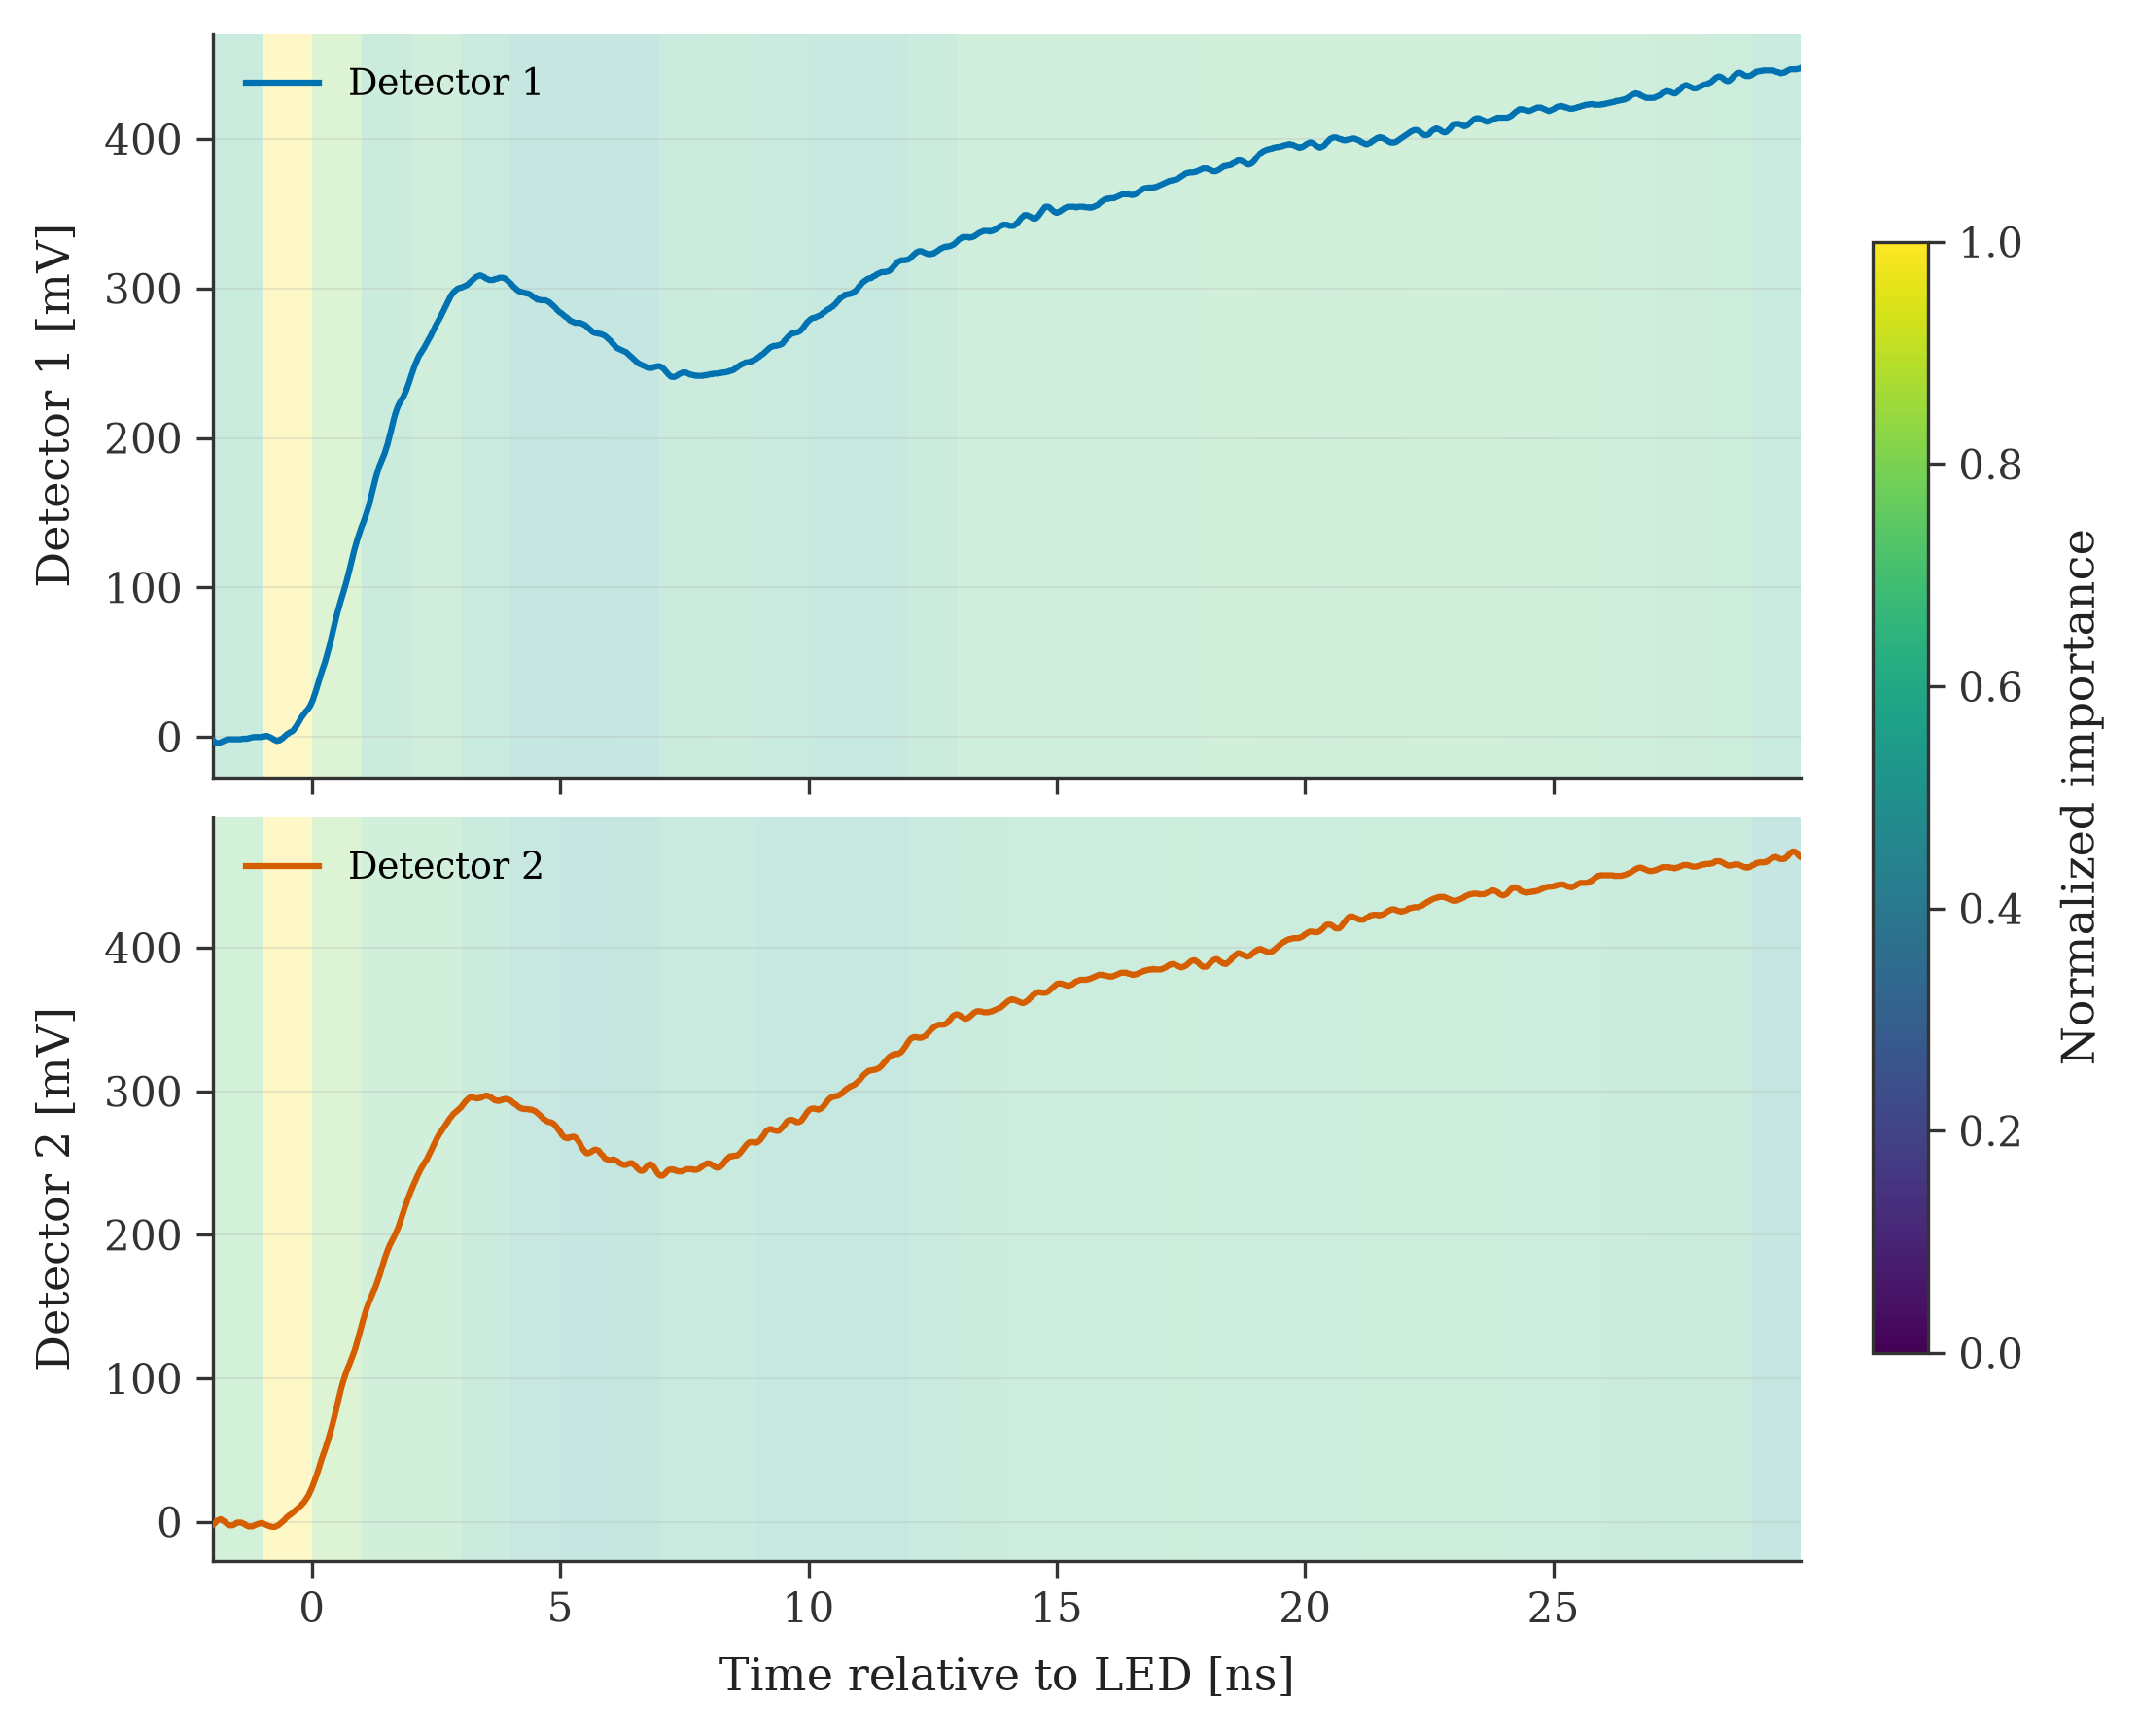
\includegraphics[width=\columnwidth]{figures/xai/energy_FBK.png}
\caption{FBK energy waveforms, wide window: temporal occlusion sensitivity
of the estimator with the lowest observed test CTR (direct MiniRocket), shown against the
two detector waveforms.}
\label{fig:fbk-energy-wide-xai}
\end{figure}

\begin{figure}[tbp]
\centering
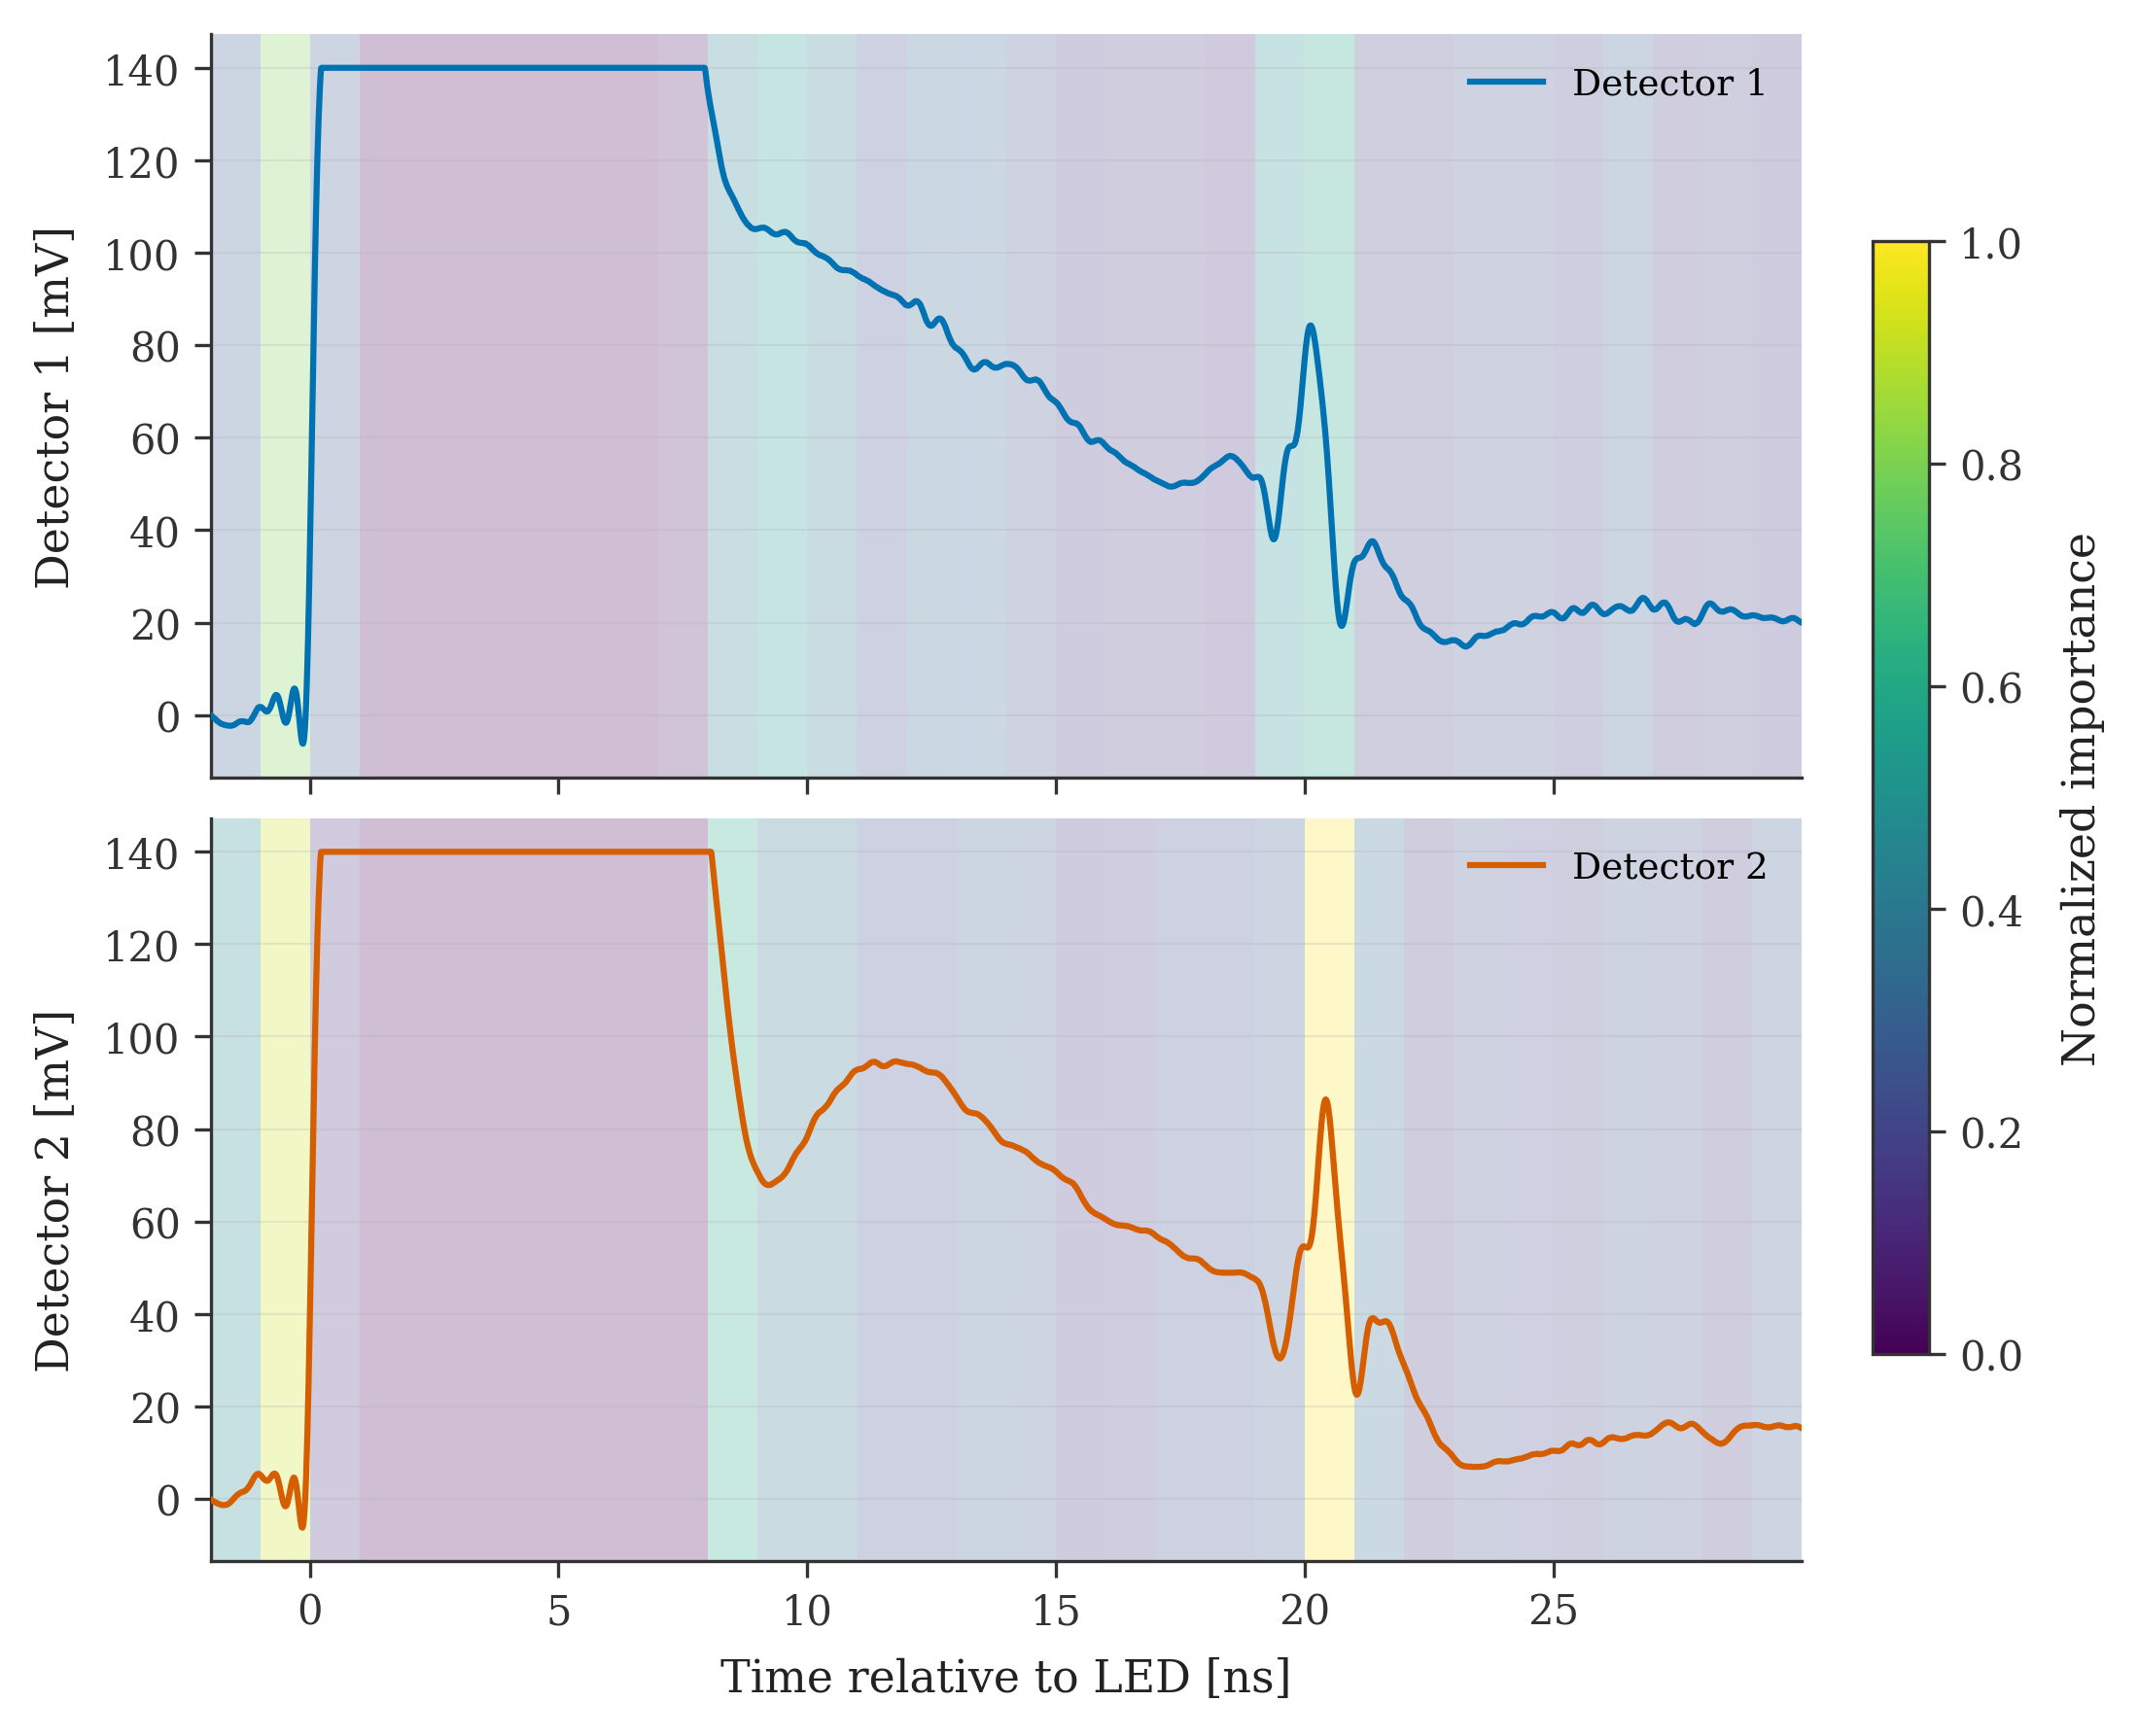
\includegraphics[width=\columnwidth]{figures/xai/timing_FBK.png}
\caption{FBK timing waveforms, wide window: temporal occlusion sensitivity
of the estimator with the lowest observed test CTR (direct linear ridge), shown against the
two detector waveforms.}
\label{fig:fbk-timing-wide-xai}
\end{figure}

\begin{figure}[tbp]
\centering
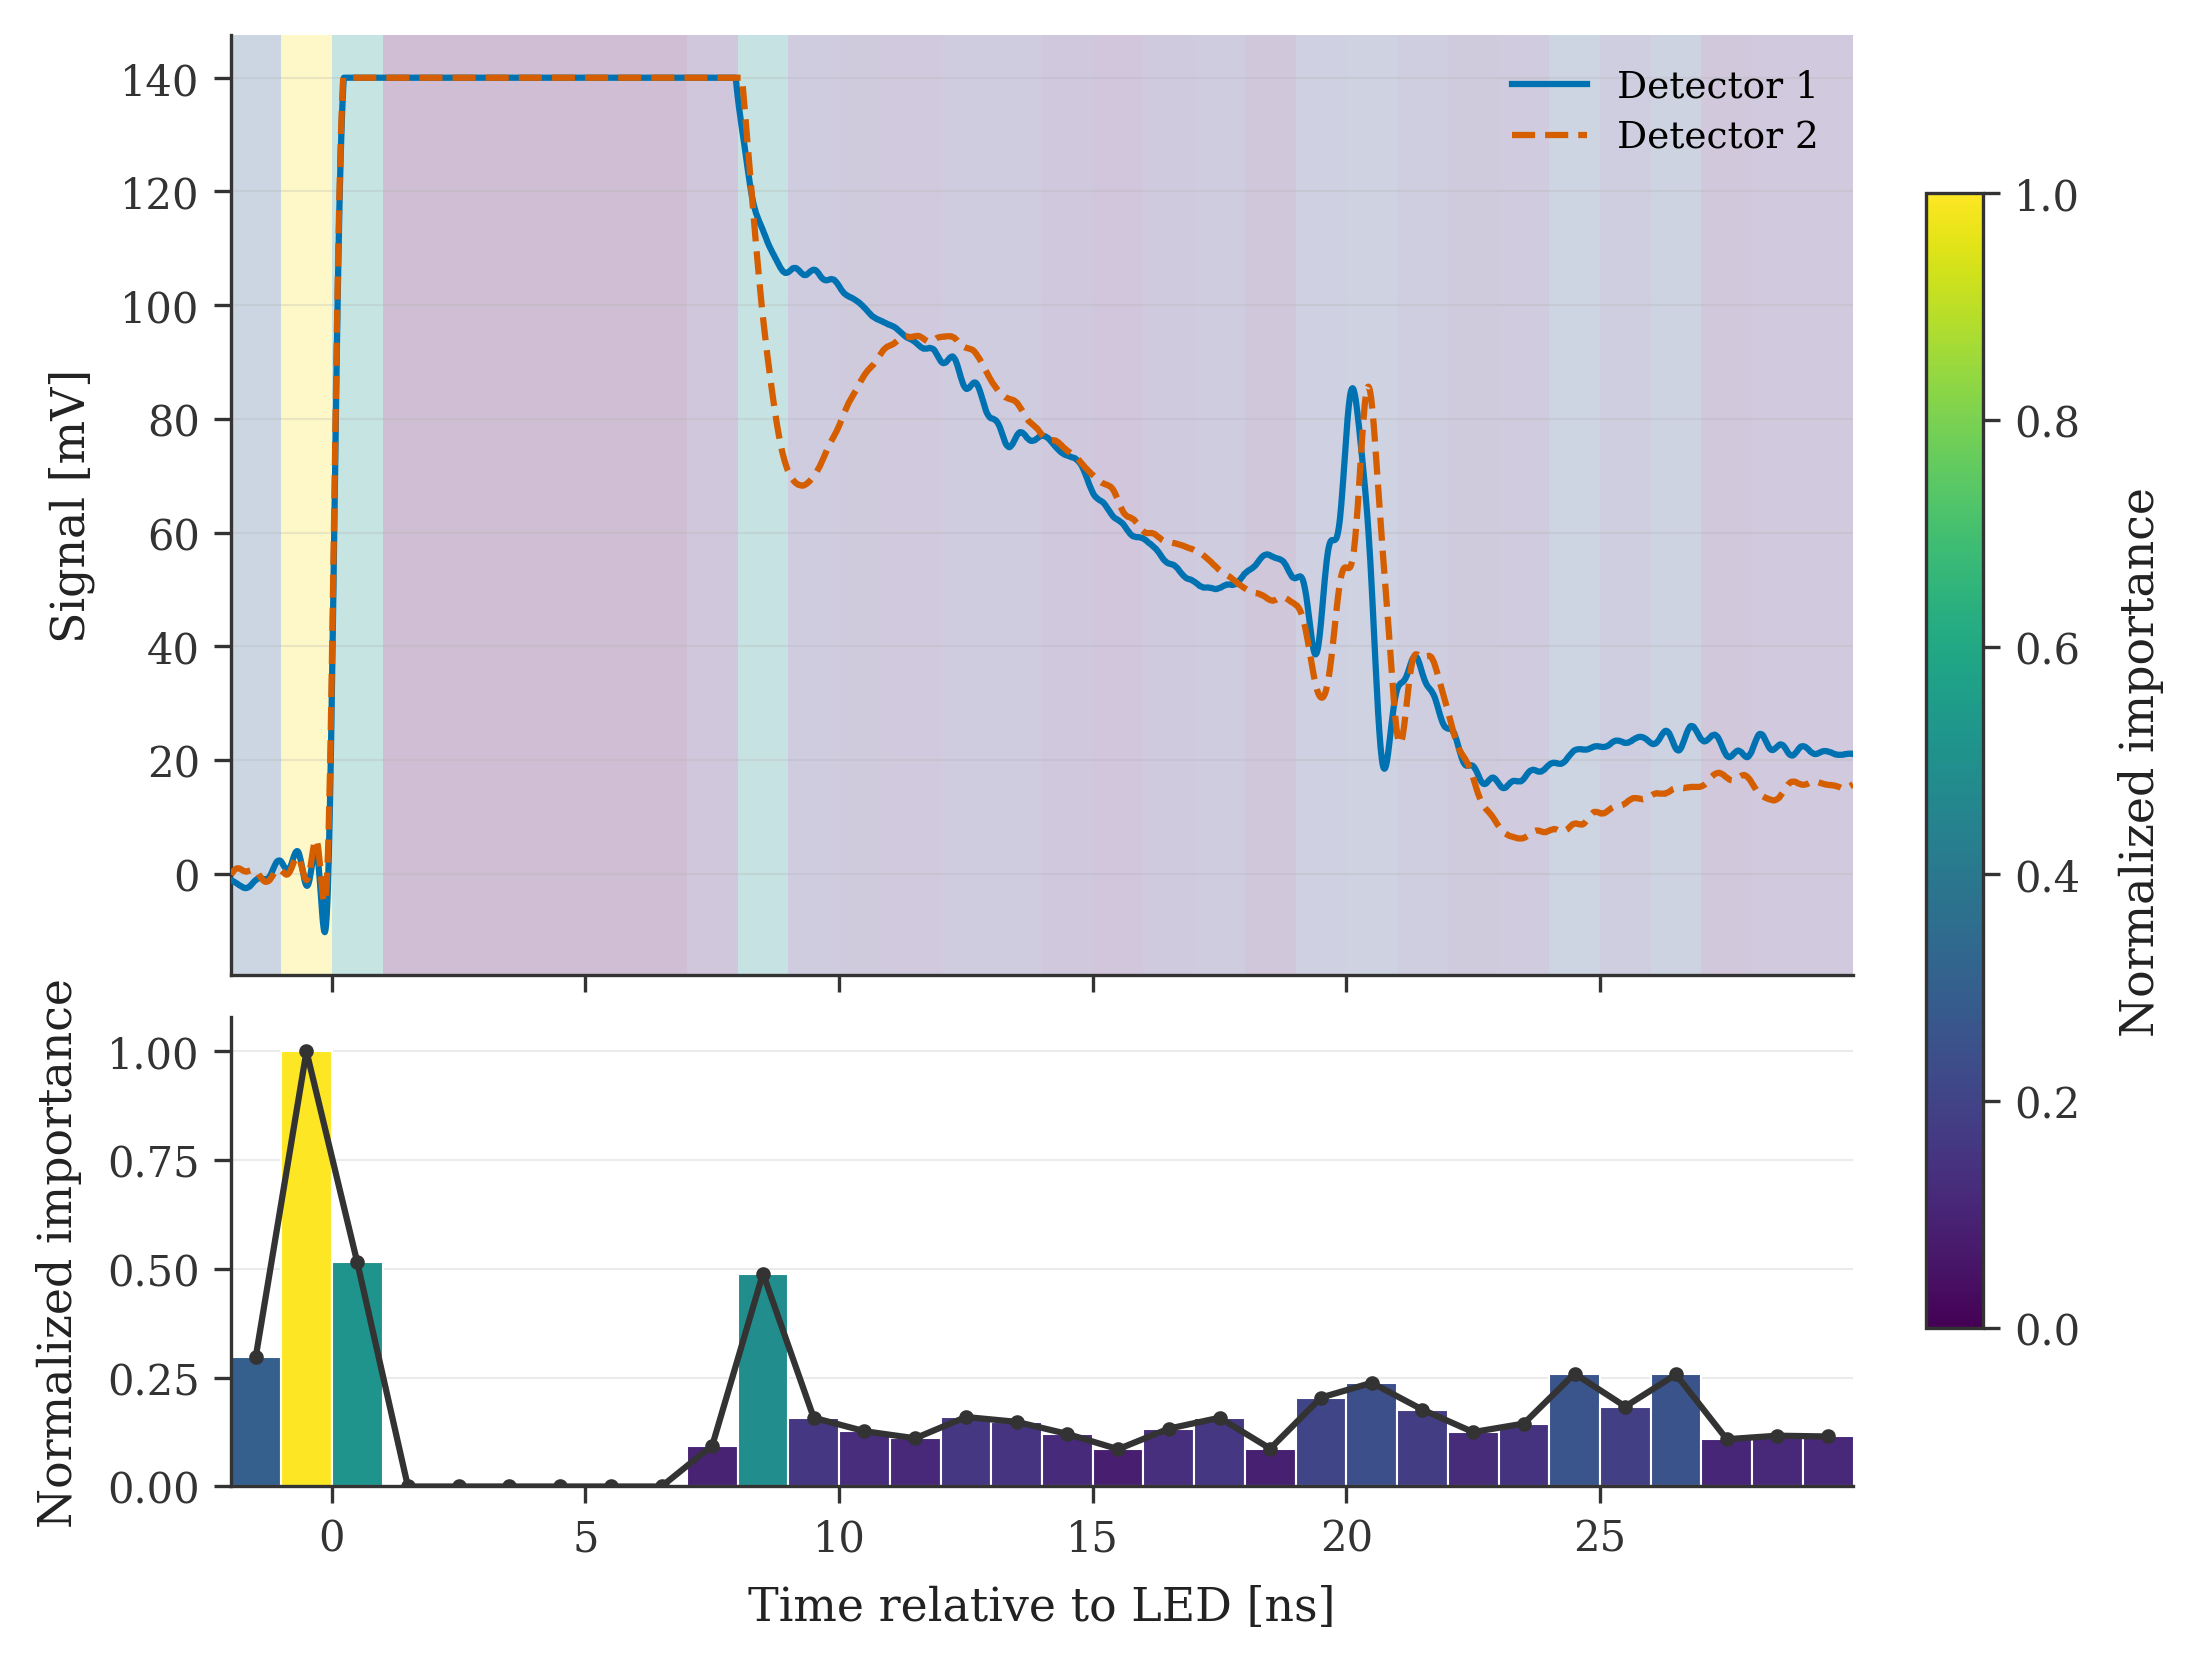
\includegraphics[width=\columnwidth]{figures/xai/timing_FBK_shared.png}
\caption{FBK timing waveforms, wide window: shared MiniRocket temporal
occlusion sensitivity, included as an additional model comparison rather
than the lowest-observed-CTR estimator. The lower panel displays the normalized
sensitivity profile, including its secondary peak near $20$--$21\,\mathrm{ns}$.}
\label{fig:fbk-timing-wide-shared-xai}
\end{figure}

\subsection{Comparison across waveform modes}
Across both boards, the dedicated second-stage timing signals provide
substantially better timing resolution than the first-stage energy signals,
both before and after waveform-based correction. In the wide-window
comparisons, the minimum energy CTRs are $105.3$ and $111.0\,\mathrm{ps}$
for UC and FBK, respectively, compared with $52.9$ and
$54.4\,\mathrm{ps}$ for timing waveforms
(Tables~\ref{tab:uc-energy-wide}, \ref{tab:uc-timing-wide},
\ref{tab:fbk-energy-wide}, and~\ref{tab:fbk-timing-wide}).
Importantly, waveform-based correction still provides an additional
improvement when applied to the timing-optimized second-stage signal.
The two boards reach a similar corrected timing performance despite
their different LED references and front-end implementations.

\section{Conclusions}
\subsection{CTR improvement}
Waveform-based correction substantially improved leading-edge 
timing on the first-stage energy signals of both boards. 
The test CTR was reduced by more than $20\%$ 
even with the short Onishi-inspired window, with reductions 
reaching approximately $25\%$ when the wider window was used. 
The strong performance of the
Onishi-inspired CNN in the short-window energy comparisons is
consistent with previous waveform-based LED correction
studies~\cite{onishi2022,loignon2025}.

\subsection{Shared detector-level models}
The detector-shared formulation retained competitive timing
performance without using separate detector-specific scoring
functions. Across the eight board, mode, and window comparisons, 
the best detector-shared estimator achieved a test CTR within 
$2\%$ of the overall best in six cases, with a maximum relative 
difference of approximately $3.5\%$. 
This shows that most of the achievable timing correction can be 
retained using a shared detector-level model, without requiring 
separate parameters for each detector.

\subsection{Model comparison}
CNN and MLP approaches did not consistently outperform linear 
regression, despite the successful application of CNNs in previous 
waveform-based timing studies~\cite{onishi2022,loignon2025}. 
In all four wide-window comparisons, the lowest test CTR 
was achieved either by linear ridge regression or by MiniRocket 
features followed by ridge regression. 
This suggests that much of the waveform-dependent timing 
correction can be captured by linear regression or linear 
combinations of extracted features, without requiring 
end-to-end nonlinear neural networks. The marked FBK
energy-wide shared-CNN failure also highlights a practical advantage
of the ridge-based estimators: for fixed input features, ridge
regression has a convex objective and is not subject to the
initialization-dependent optimization of the neural models. Together
with their competitive timing performance, this makes the linear
approaches particularly attractive for this correction task.

\subsection{Window length and XAI}
Extending the waveform window consistently improved
 the best timing resolution on both boards, 
 with a particularly important effect on the timing signals, 
 where short windows provided limited correction. 
 Temporal occlusion analysis showed that energy-channel 
 models relied primarily on the region around the LED crossing,  
 while timing-channel models were also sensitive to later waveform structures. 
 This was especially evident for the FBK board, where a 
 pronounced secondary sensitivity peak appeared around $20\,\mathrm{ns}$. 
 These findings support the usefulness of waveform information 
 beyond the rising edge.

 \subsection{Final considerations}
 Despite ML correction, the second-stage timing signals achieved 
 approximately twice the timing resolution of the first-stage energy signals, 
 highlighting that waveform-based correction cannot fully compensate for differences 
 in analog readout quality. 
 Nevertheless, ML consistently improved LED timing, with both boards reaching similar 
 corrected CTRs of approximately $53$–$54\,\mathrm{ps}$ despite different amplification 
 electronics and LED thresholds. 
 This convergence suggests that the remaining timing uncertainty may be dominated by 
 physical effects common to the detectors that cannot be recovered from the available 
 waveform information, although this hypothesis requires further investigation.

\appendix
\section{Model architectures and training settings}
\label{app:spaces}
The model families represent different assumptions about how waveform
information can correct LED timing. Their detector-pair formulations are
described below; Tables~\ref{tab:space-neural-summary} and
\ref{tab:space-ridge-minirocket-summary} collect the configured search spaces.

\subsection{Linear ridge regression}
Linear models provide a computationally inexpensive baseline for testing
whether a weighted combination of waveform samples is sufficient for timing
correction. The direct estimator uses independent weights on the concatenated
detector waveforms and an intercept. The shared estimator instead applies
common weights to the sample-wise waveform difference, without an intercept,
enforcing detector-exchange antisymmetry:
\begin{equation}
h(s_1,s_2)=\mathbf{w}^{T}(s_1-s_2)
=\mathbf{w}^{T}s_1-\mathbf{w}^{T}s_2.
\end{equation}
Ridge regularization limits sensitivity to highly correlated samples. Its
strength is selected by internal leave-one-out cross-validation minimizing
mean squared error (MSE), rather than the outer CTR-based selection.

\subsection{Convolutional neural networks}
Convolutional neural networks (CNNs) are established waveform-timing models,
including for LED correction~\cite{onishi2022,loignon2025}. Their temporal
filters exploit local waveform structure with weights shared across sample
positions. The Onishi-inspired direct CNN combines the detector dimension in
the first convolution and predicts a joint correction. The independent CNN
uses separately parameterized detector scorers, whereas the shared CNN uses
one common scorer for both detector signals.

\subsection{Multilayer perceptrons}
The direct dense MLP performs nonlinear regression on the concatenated
waveforms. The shared MLP applies the same nonlinear scorer to both detector
signals and subtracts the two outputs,
\begin{equation}
h_\theta(s_1,s_2)=g_\theta(s_1)-g_\theta(s_2).
\end{equation}
The shared locally connected MLP preserves temporal neighborhoods without
sharing filters across positions. This is useful for LED-aligned waveforms,
where temporal position itself is informative, and provides an intermediate
assumption between dense and convolutional processing~\cite{elsayed2020}.

\subsection{MiniRocket feature regression}
MiniRocket is an efficient, largely deterministic convolutional feature
transformation developed for time-series classification~\cite{minirocket2021}.
Here its features are used for timing-error regression with ridge
regularization. The direct model transforms the waveform pair jointly; the
shared model applies the same univariate transform to both detector signals
and regresses on their feature difference.

\subsection{Training and configured spaces}
Dense MLPs, the locally connected MLP and temporal CNNs use at most 300
epochs, an internal holdout fraction of 0.2, loss-stop patience of 10 epochs,
a minimum loss improvement of $0.1\,\mathrm{ps}$, gradient clipping at 10,
and a gradient-stop threshold of $10^{-6}$ with patience 4. The Onishi-inspired
CNN instead uses a fixed 100-epoch schedule with learning-rate reductions at
epochs 30 and 60. Hyperparameters for neural and MiniRocket models are selected
from the training acquisition using mean held-out CTR in the three common
outer folds; the two linear ridge estimators use internal leave-one-out
cross-validation on MSE.

\subsection{Software libraries}
Table~\ref{tab:model-libraries} summarizes the principal scientific software
and declared minimum versions.
\begin{table}[tbp]
\centering
\scriptsize
\begin{tabularx}{\columnwidth}{@{}lclX@{}}
\toprule
Library & Min. & Role \\
\midrule
PyTorch & 2.2 & Neural models \\
scikit-learn & 1.4 & Ridge CV and scaling \\
sktime & 0.35 & MiniRocket transforms \\
NumPy & 1.26 & Waveform and bootstrap operations \\
SciPy & 1.11 & Numerical routines and Gaussian fits \\
Matplotlib & 3.8 & Figures \\
pandas & 2.1 & Tabular data and transformed features \\
Optuna & 4.0 & Optional adaptive parameter proposal \\
\bottomrule
\end{tabularx}
\caption{Principal scientific software and declared minimum versions.}
\label{tab:model-libraries}
\end{table}



\begin{table*}[tbp]
\centering
\footnotesize
\begin{tabularx}{\textwidth}{@{}p{0.08\textwidth}Xp{0.21\textwidth}p{0.12\textwidth}p{0.18\textwidth}@{}}
\toprule
Code & Architecture & Learning rate & Batch size & Optimizer / schedule \\
\midrule
S-MLP
& $\{[16],[128],[128,64],[16,16,16]\}$
& $\{10^{-2},10^{-3},10^{-4},10^{-5}\}$
& 32
& Nesterov SGD \\

D-MLP
& $\{[16],[128],[128,64],[16,16,16]\}$
& $\{10^{-2},10^{-3},10^{-4},10^{-5}\}$
& 32
& Adam \\

S-LCM
& Dense [128]; local kernels $(3,3)$, strides $(1,1)$; correction bound $500\,\mathrm{ps}$
& $\{10^{-2},10^{-3},10^{-4},10^{-5}\}$
& $\{32,128\}$
& Adam \\

S-CNN
& Channels [16,32]; kernels [5,3]; dense 64
& $\{10^{-3},10^{-4},10^{-5}\}$
& $\{32,128\}$
& Adam \\

D-CNN
& Channels [16,32]; kernels [5,3]; dense 64
& $\{10^{-3},10^{-4},10^{-5}\}$
& $\{32,128\}$
& Adam \\

D-ONI
& Channels [32,64]; kernels [5,3]; dense 256
& $\{10^{-3},10^{-4},10^{-5}\}$
& $\{32,128\}$
& Adam; 100 epochs, LR drops at 30/60 \\
\bottomrule
\end{tabularx}
\caption{Configured neural-model search spaces. Model codes are defined in
Table~\ref{tab:model-inventory}. All models use ReLU activations; training
settings shared across models are given in the text.}
\label{tab:space-neural-summary}
\end{table*}
\begin{table*}[tbp]
\centering
\scriptsize
\begin{tabularx}{\textwidth}{@{}llXXl@{}}
\toprule
Code & Estimator & Feature / regularization space & Selection & Intercept \\
\midrule
S-LIN & Shared linear ridge & 50 log-spaced ridge strengths from $10^{-8}$ to $10^{3}$ & Internal leave-one-out CV; MSE & None \\
D-LIN & Direct linear ridge & 50 log-spaced ridge strengths from $10^{-8}$ to $10^{3}$ & Internal leave-one-out CV; MSE & Included \\
S-MR & Shared MiniRocket + ridge & 10000 requested features; ridge $\alpha\in\{0.1,0.3,1,3,10,30,100,300,10^3,3\times10^3,10^4,3\times10^4,10^5,3\times10^5,10^6\}$ & Outer CV; mean CTR & None \\
D-MR & Direct MiniRocket + ridge & 10000 requested features; same ridge grid & Outer CV; mean CTR & Included \\
\bottomrule
\end{tabularx}
\caption{Configured linear and MiniRocket spaces. MiniRocket feature transforms
and scaling are fixed before supervised fitting.}
\label{tab:space-ridge-minirocket-summary}
\end{table*}



\section{Independent-test CTR comparisons}
\label{app:ctr-plots}
The following figures collect the model-wise independent-test CTR comparisons
for both waveform modes and input windows. Corresponding numerical results and
uncertainty estimates are provided in Section~\ref{sec:results-tables}.

\subsection{UC board}
\begin{figure*}[p]
\centering
\begin{subfigure}[t]{0.49\textwidth}
\centering
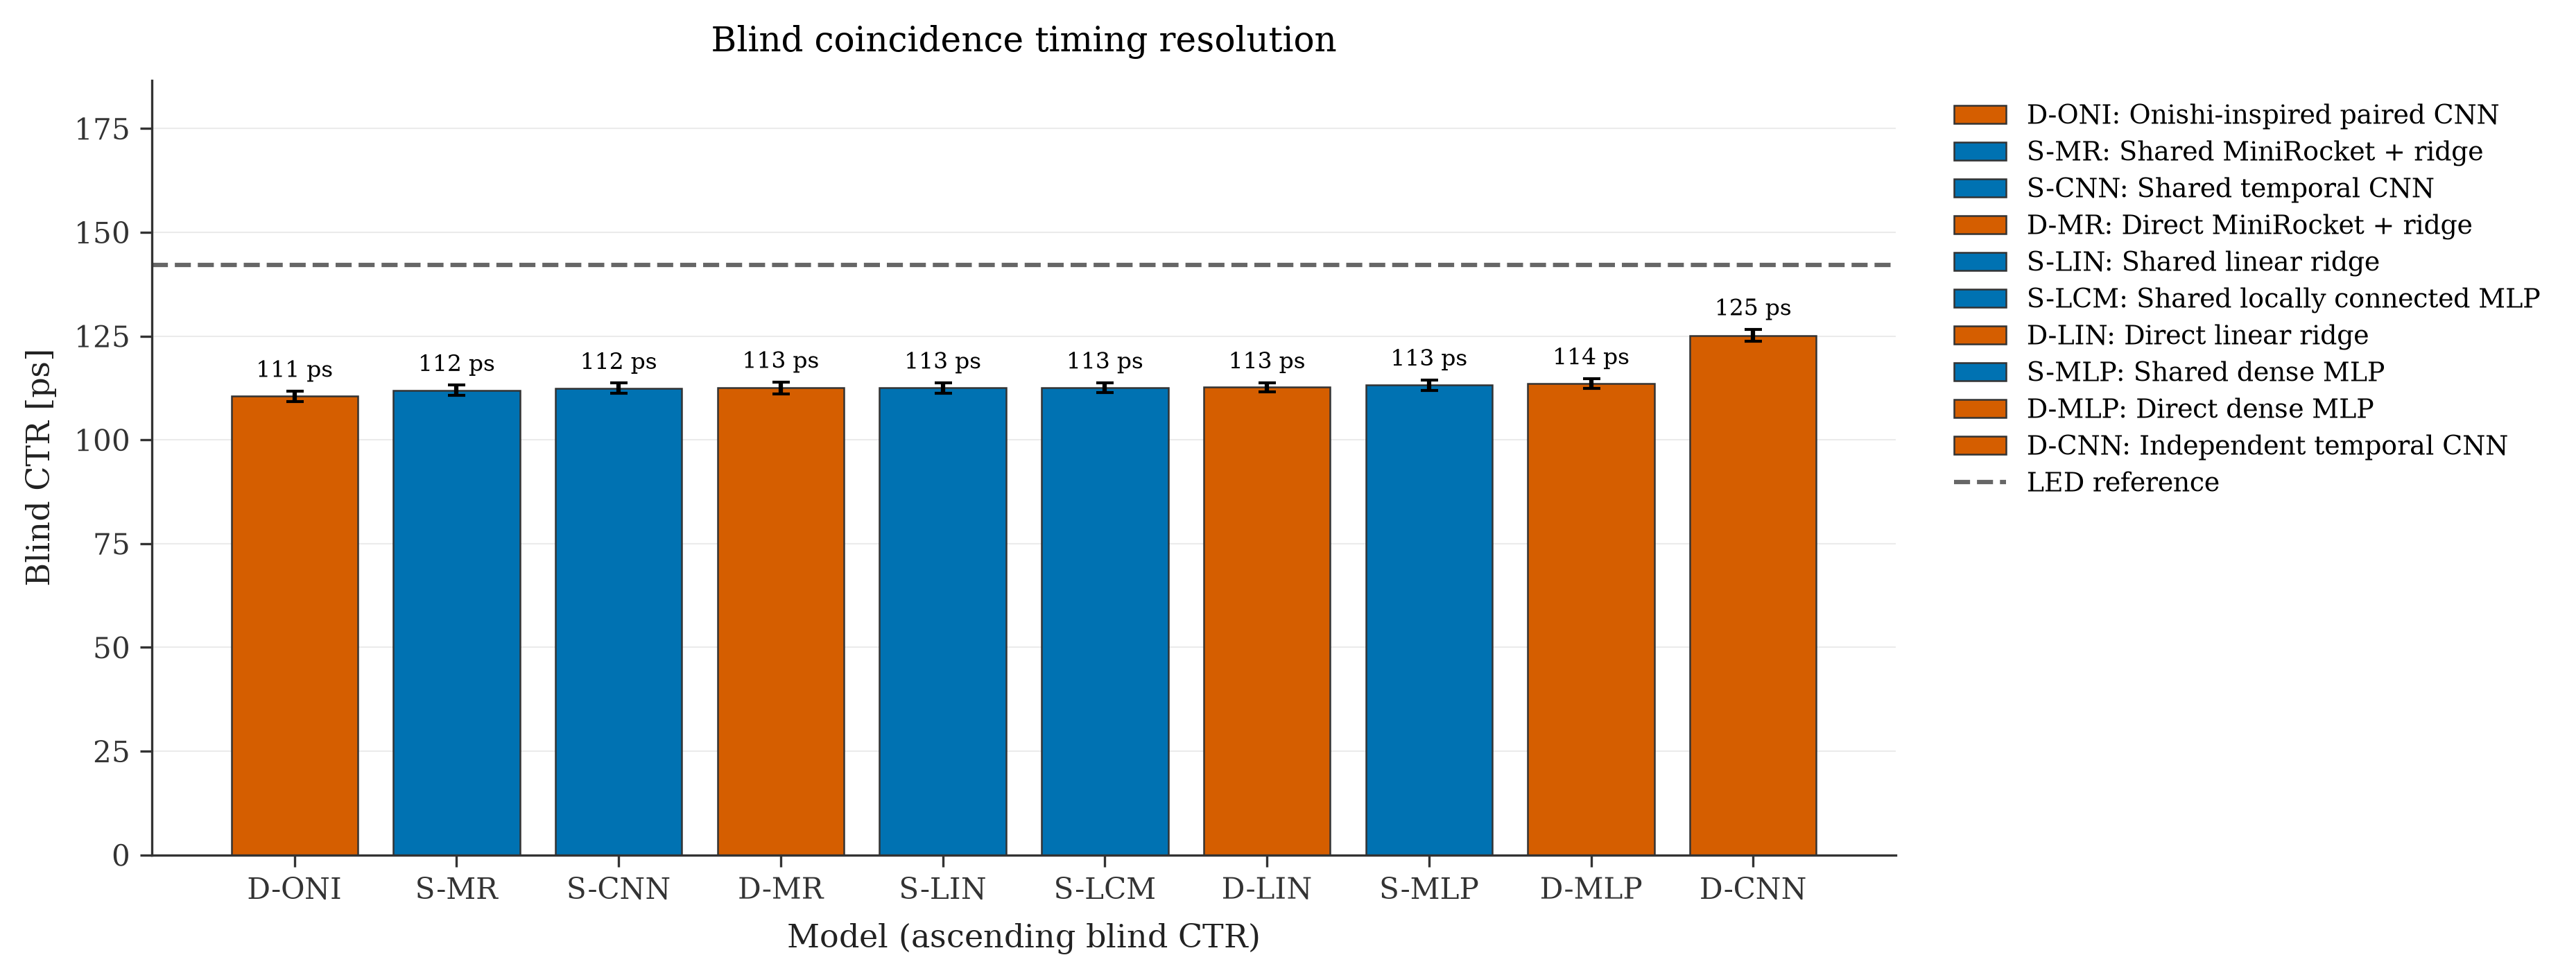
\includegraphics[width=\linewidth]{figures/results/UC/UC_energy_onishi_blind_ctr.png}
\caption{Energy, Onishi-inspired window.}
\label{fig:uc-energy-onishi-ctr}
\end{subfigure}\hfill
\begin{subfigure}[t]{0.49\textwidth}
\centering
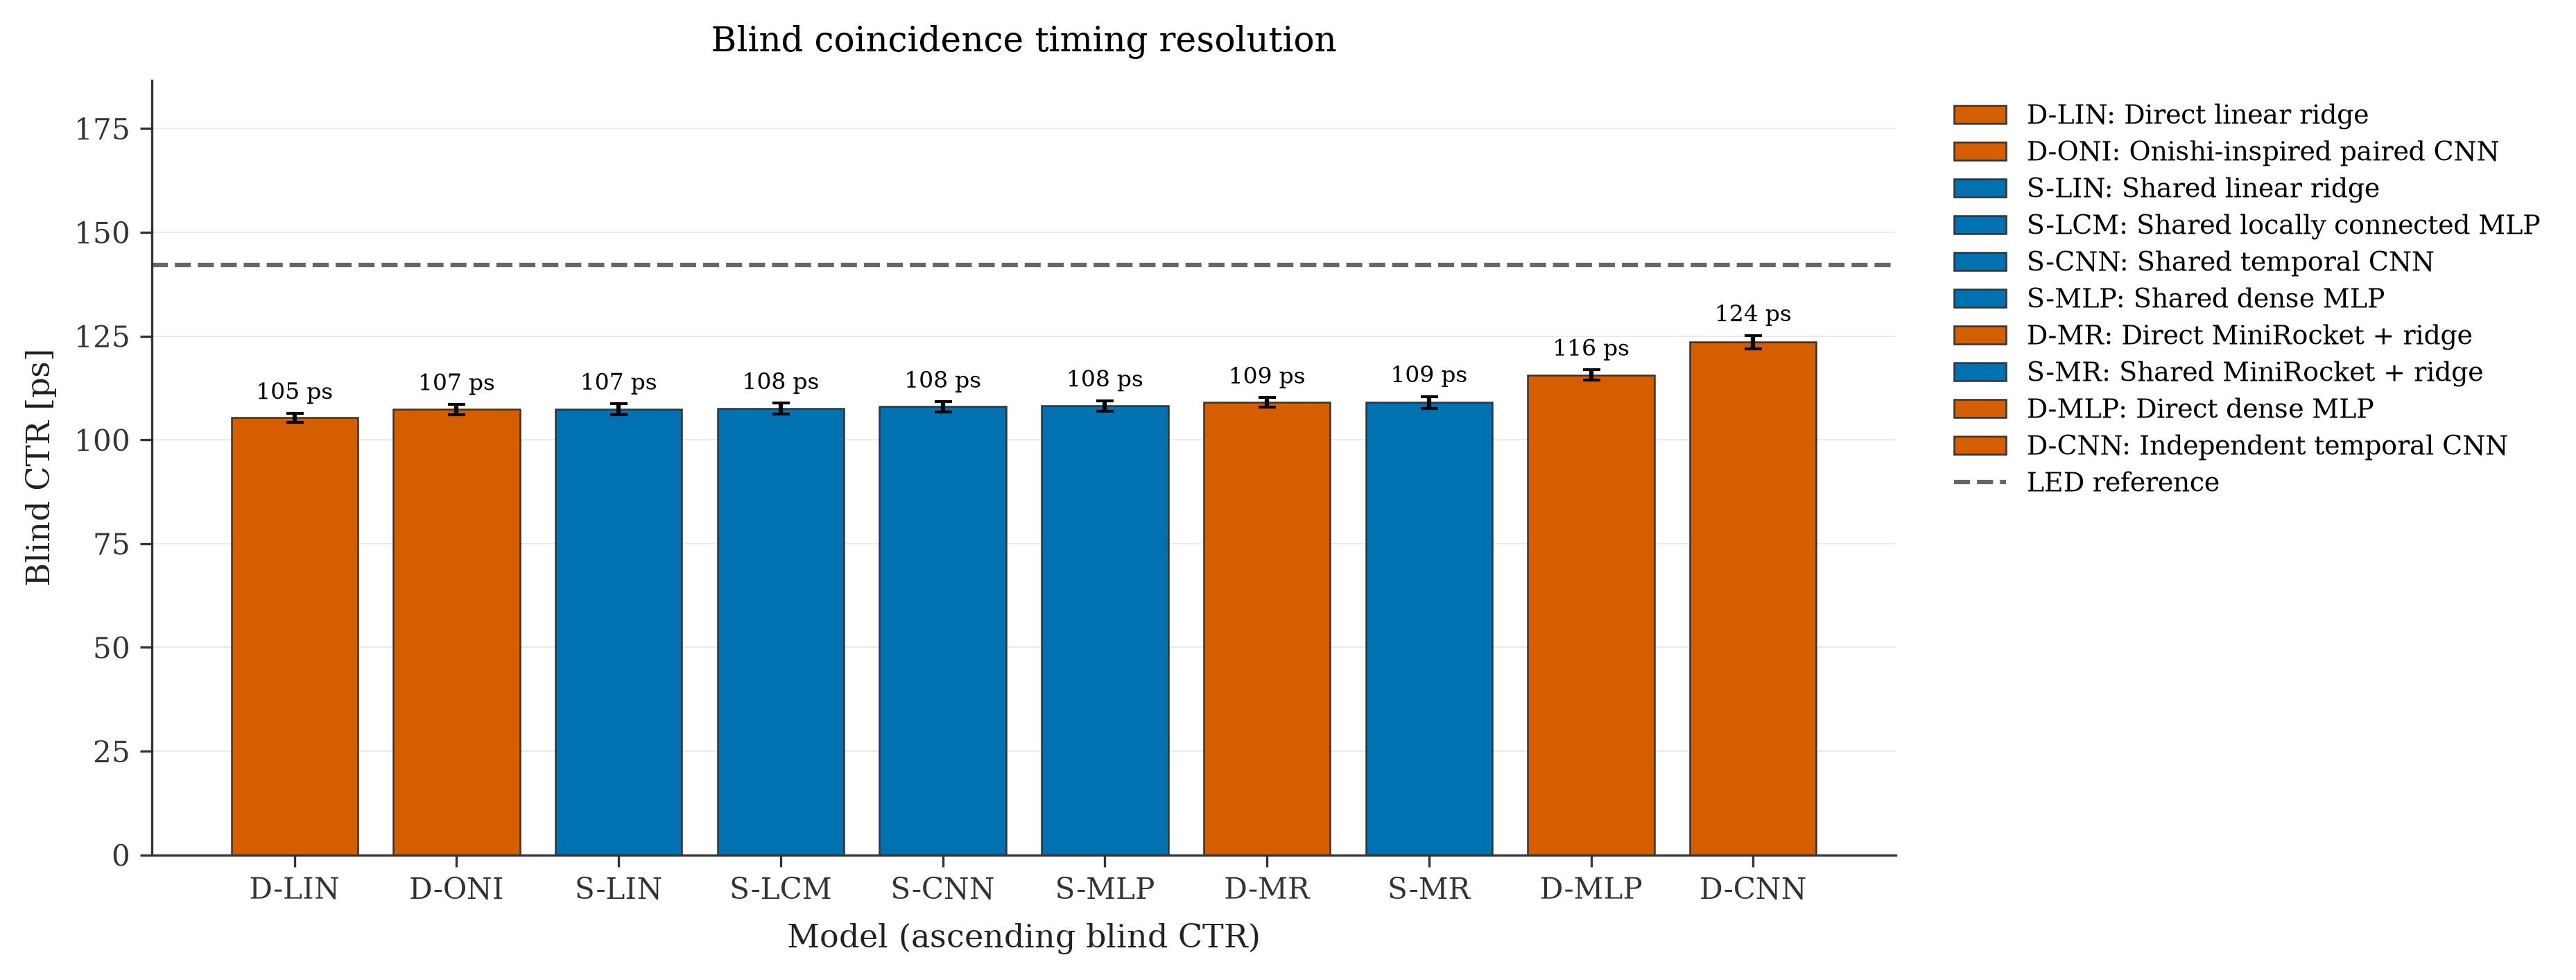
\includegraphics[width=\linewidth]{figures/results/UC/UC_energy_wide_blind_ctr.png}
\caption{Energy, wide window.}
\label{fig:uc-energy-wide-ctr}
\end{subfigure}

\medskip
\begin{subfigure}[t]{0.49\textwidth}
\centering
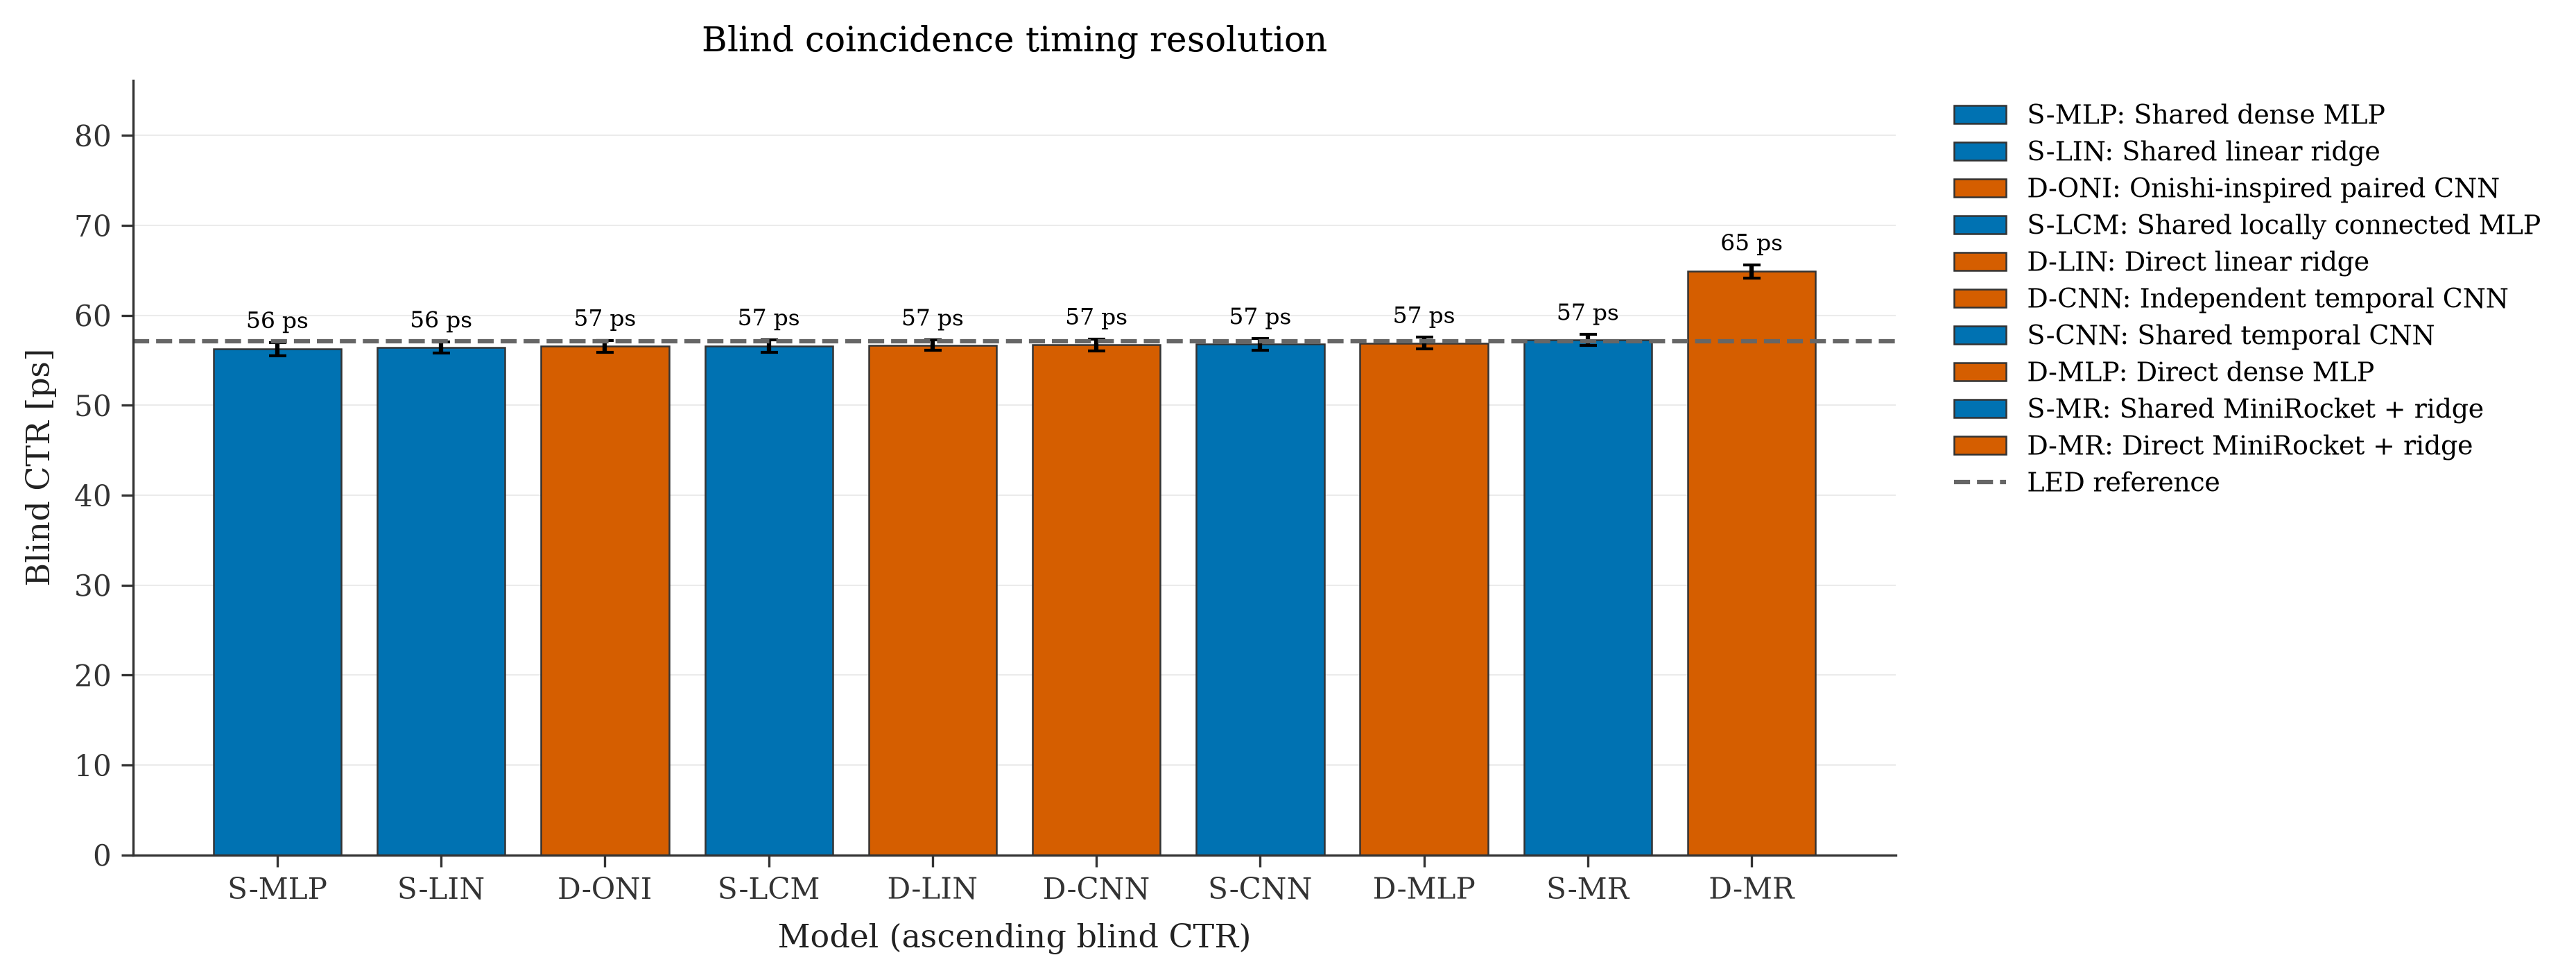
\includegraphics[width=\linewidth]{figures/results/UC/UC_timing_onishi_blind_ctr.png}
\caption{Timing, Onishi-inspired window.}
\label{fig:uc-timing-onishi-ctr}
\end{subfigure}\hfill
\begin{subfigure}[t]{0.49\textwidth}
\centering
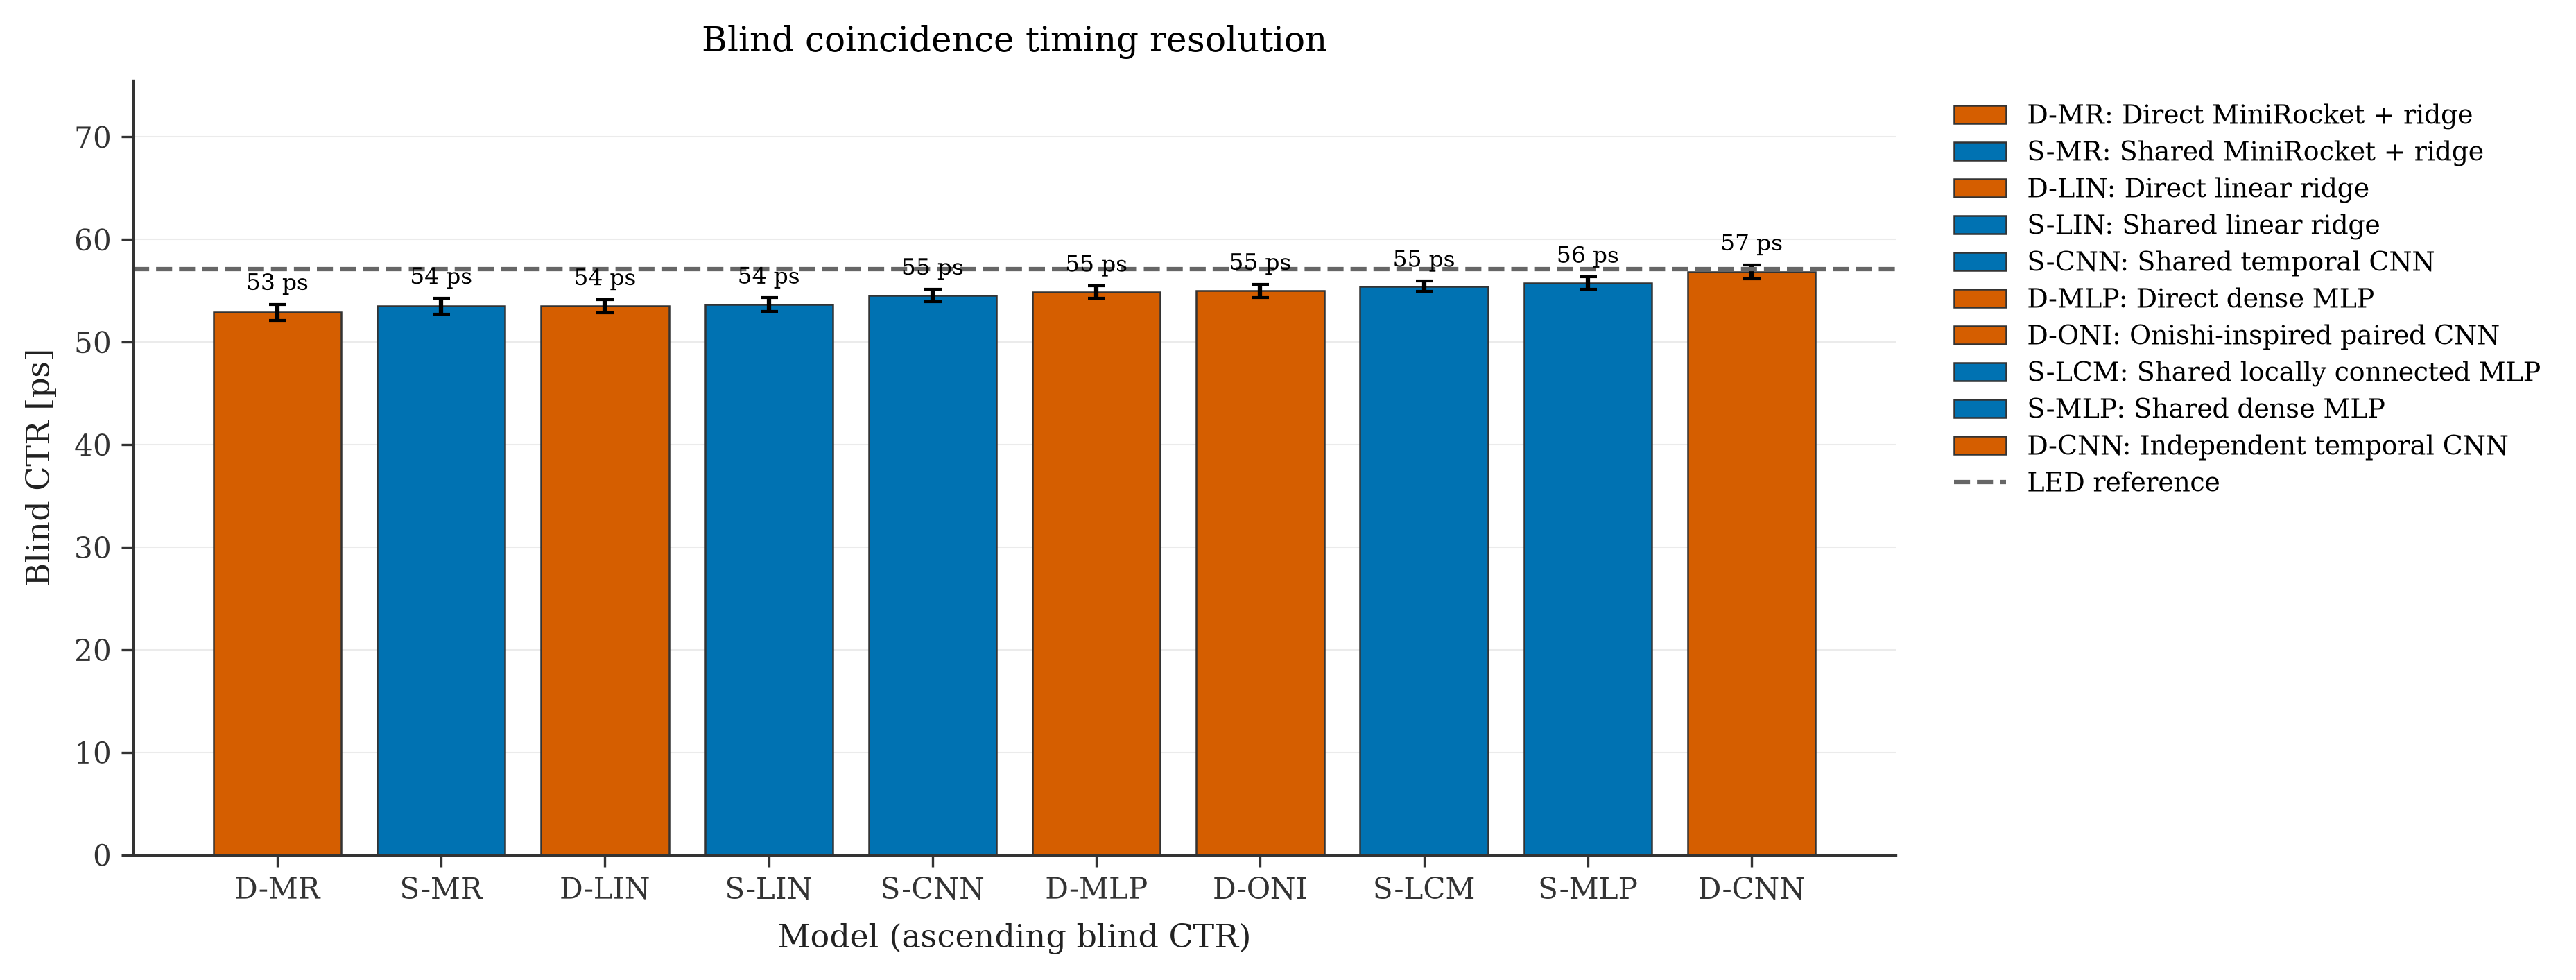
\includegraphics[width=\linewidth]{figures/results/UC/UC_timing_wide_blind_ctr.png}
\caption{Timing, wide window.}
\label{fig:uc-timing-wide-ctr}
\end{subfigure}
\caption{UC board: independent-test CTR for the compared estimators. The dashed
line denotes the LED reference and error bars indicate bootstrap standard
deviations.}
\label{fig:uc-ctr-comparison}
\end{figure*}

\subsection{FBK board}
\begin{figure*}[p]
\centering
\begin{subfigure}[t]{0.49\textwidth}
\centering
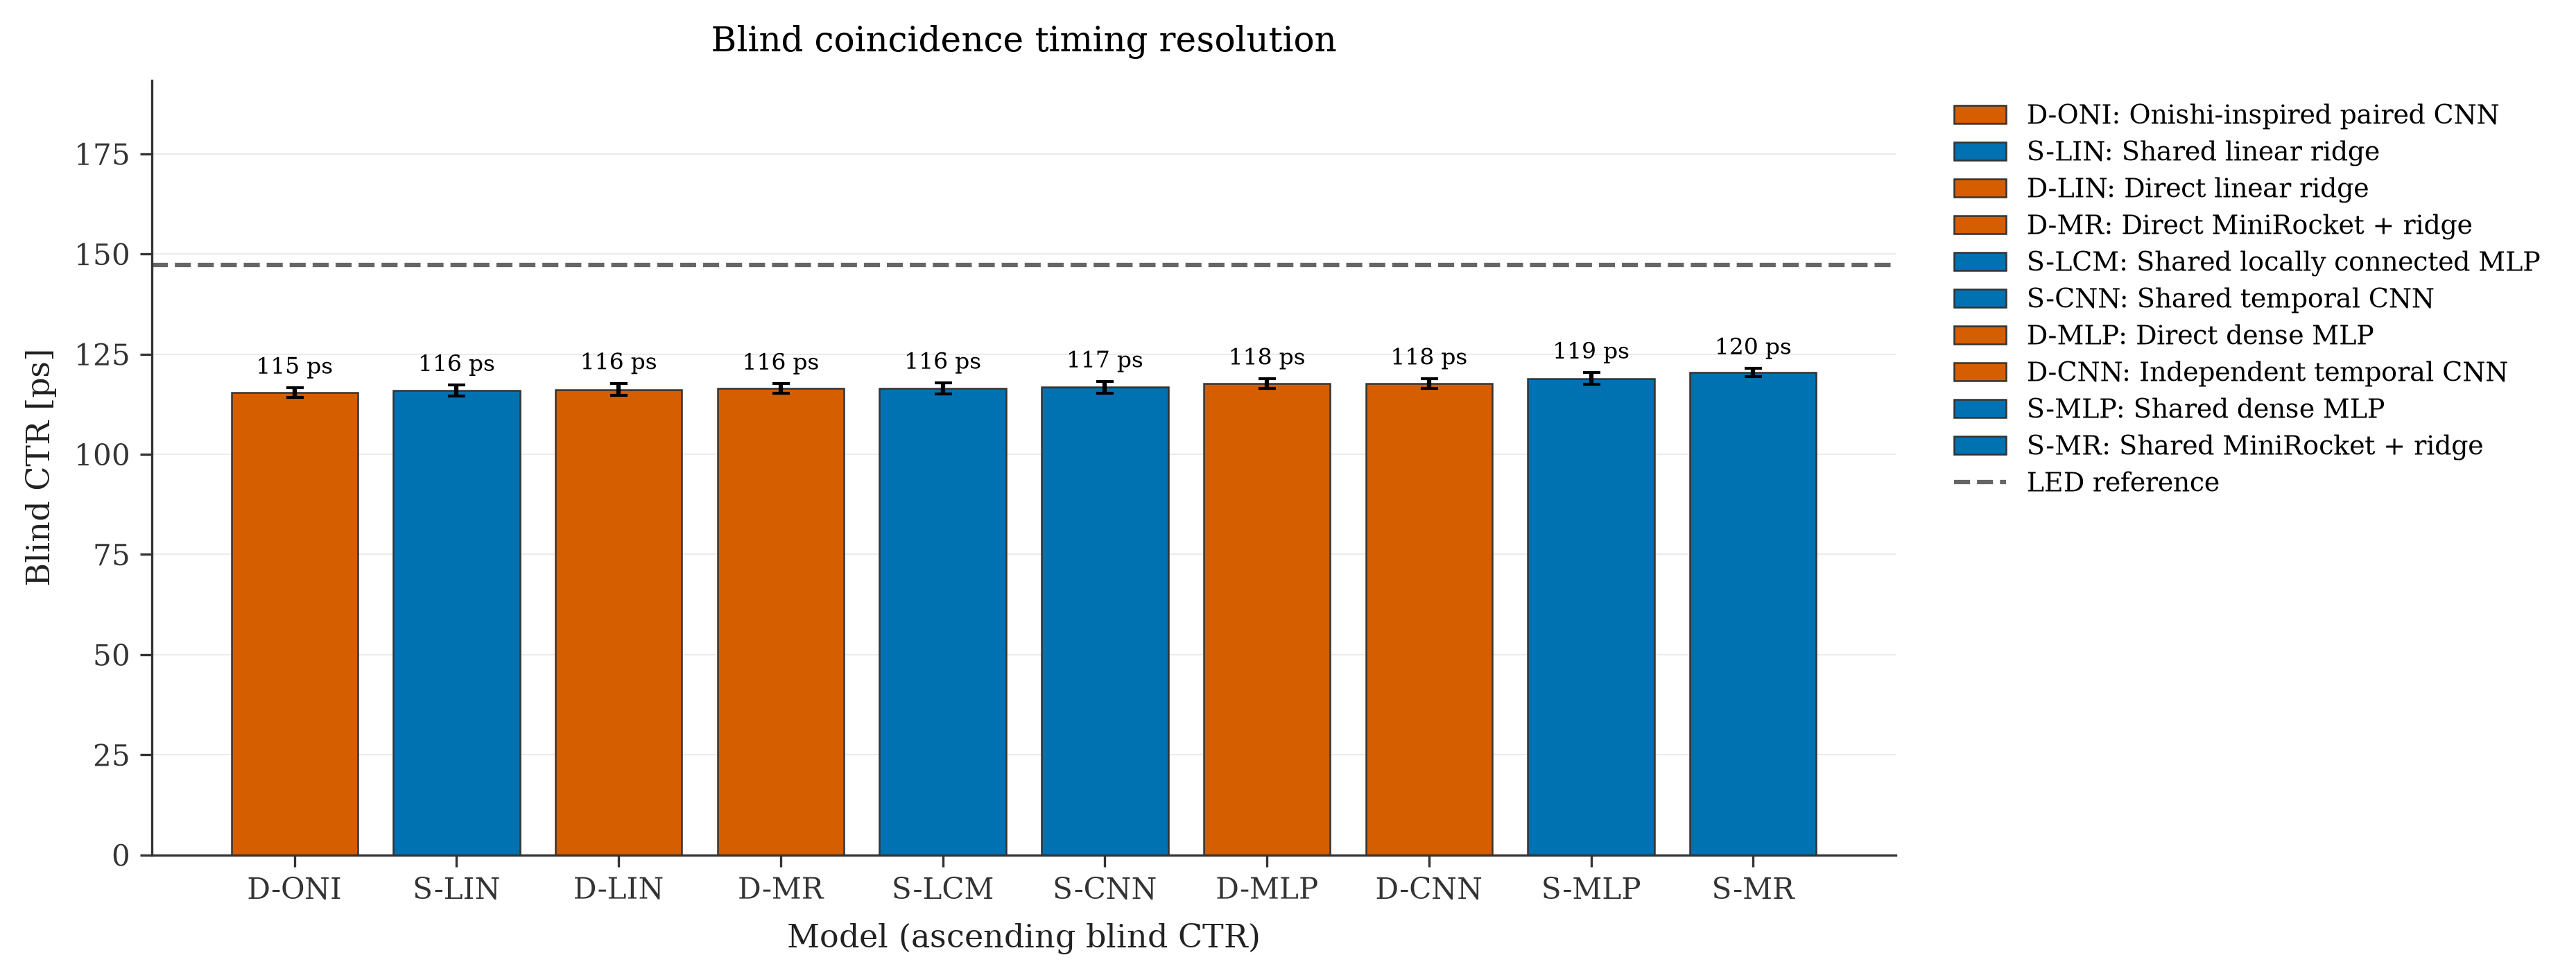
\includegraphics[width=\linewidth]{figures/results/FBK/FBK_energy_onishi_blind_ctr.png}
\caption{Energy, Onishi-inspired window.}
\label{fig:fbk-energy-onishi-ctr}
\end{subfigure}\hfill
\begin{subfigure}[t]{0.49\textwidth}
\centering
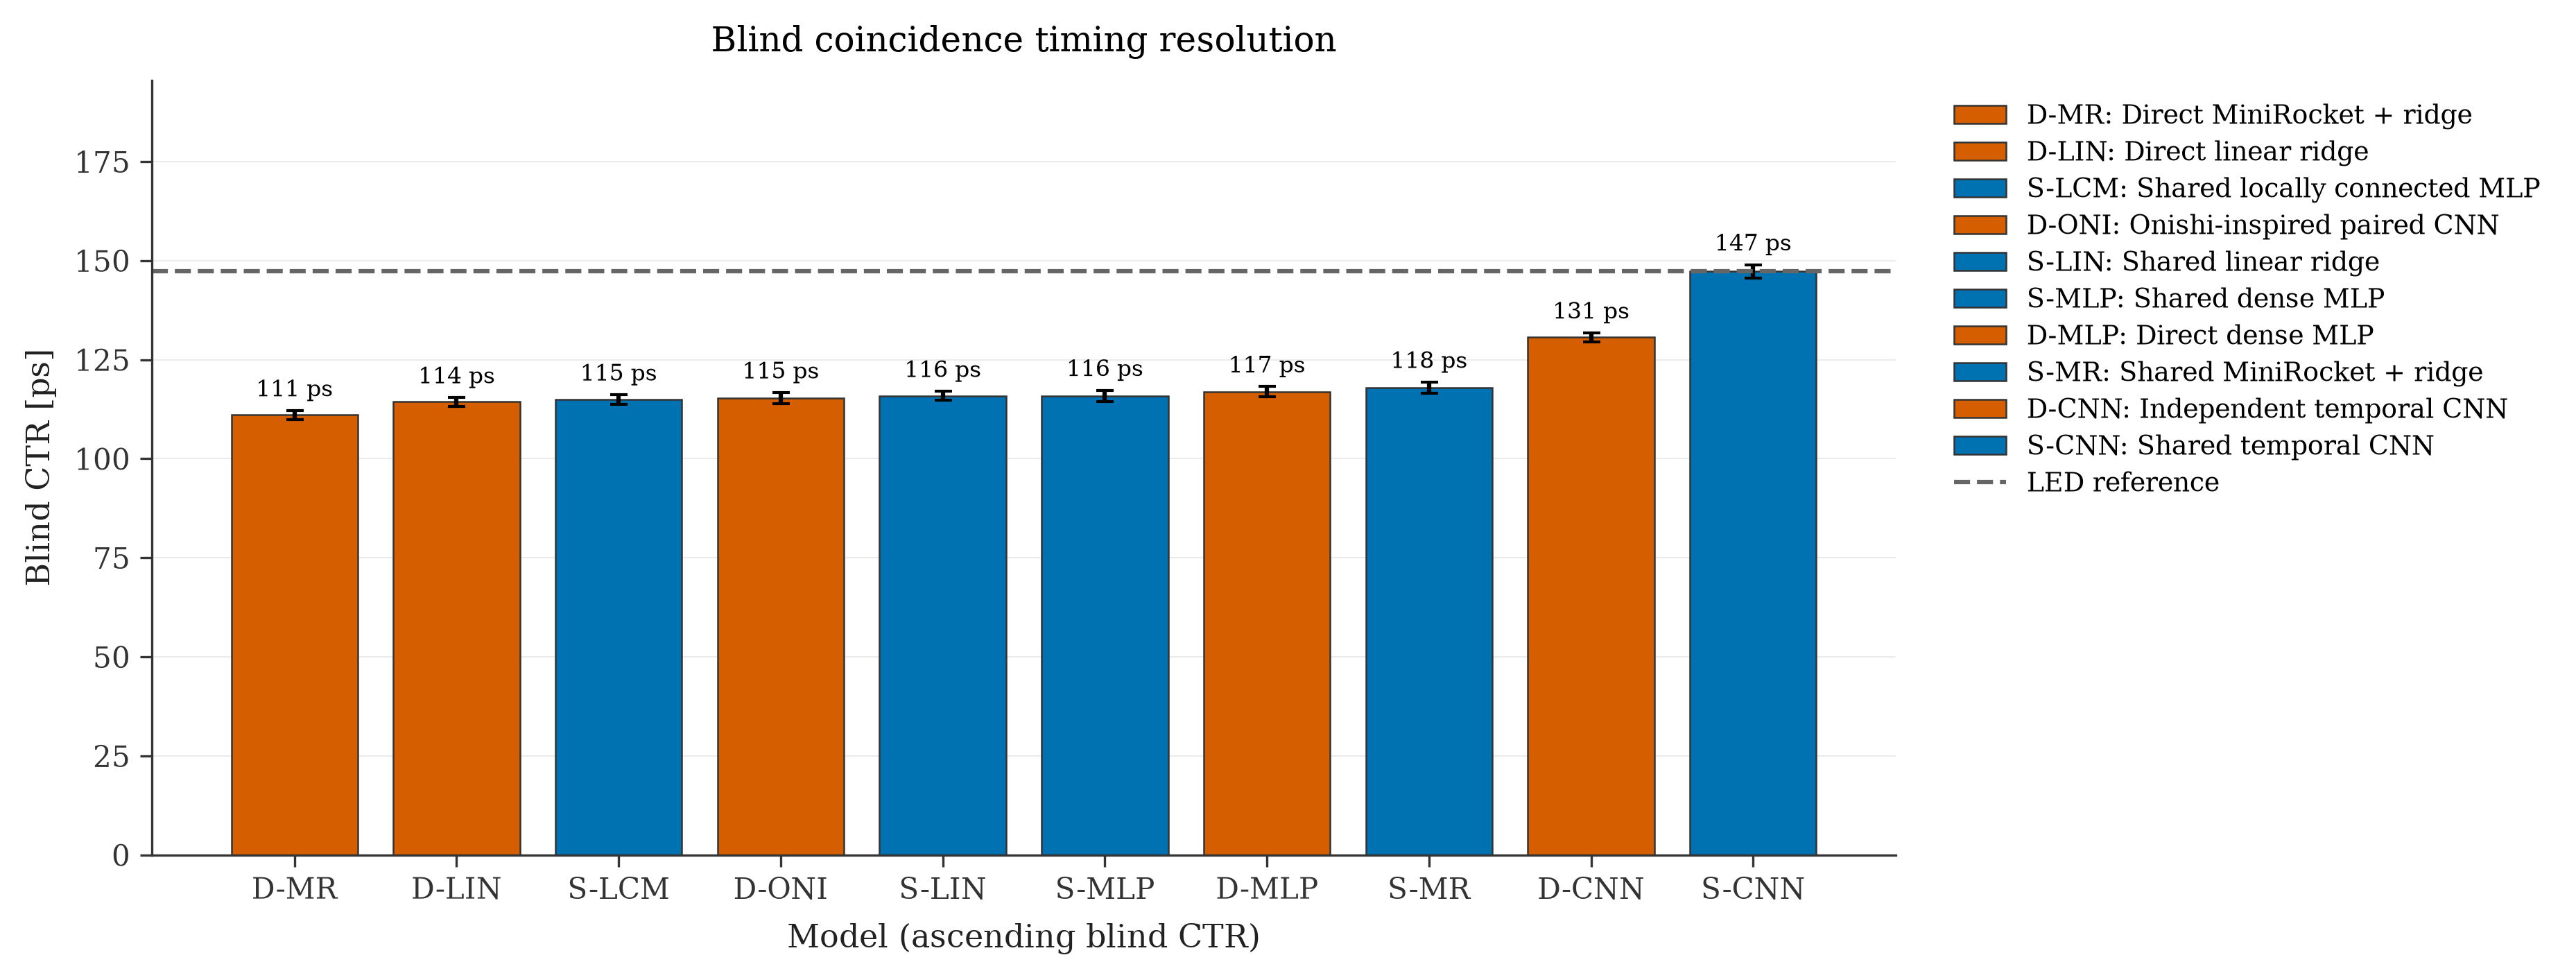
\includegraphics[width=\linewidth]{figures/results/FBK/FBK_energy_wide_blind_ctr.png}
\caption{Energy, wide window.}
\label{fig:fbk-energy-wide-ctr}
\end{subfigure}

\medskip
\begin{subfigure}[t]{0.49\textwidth}
\centering
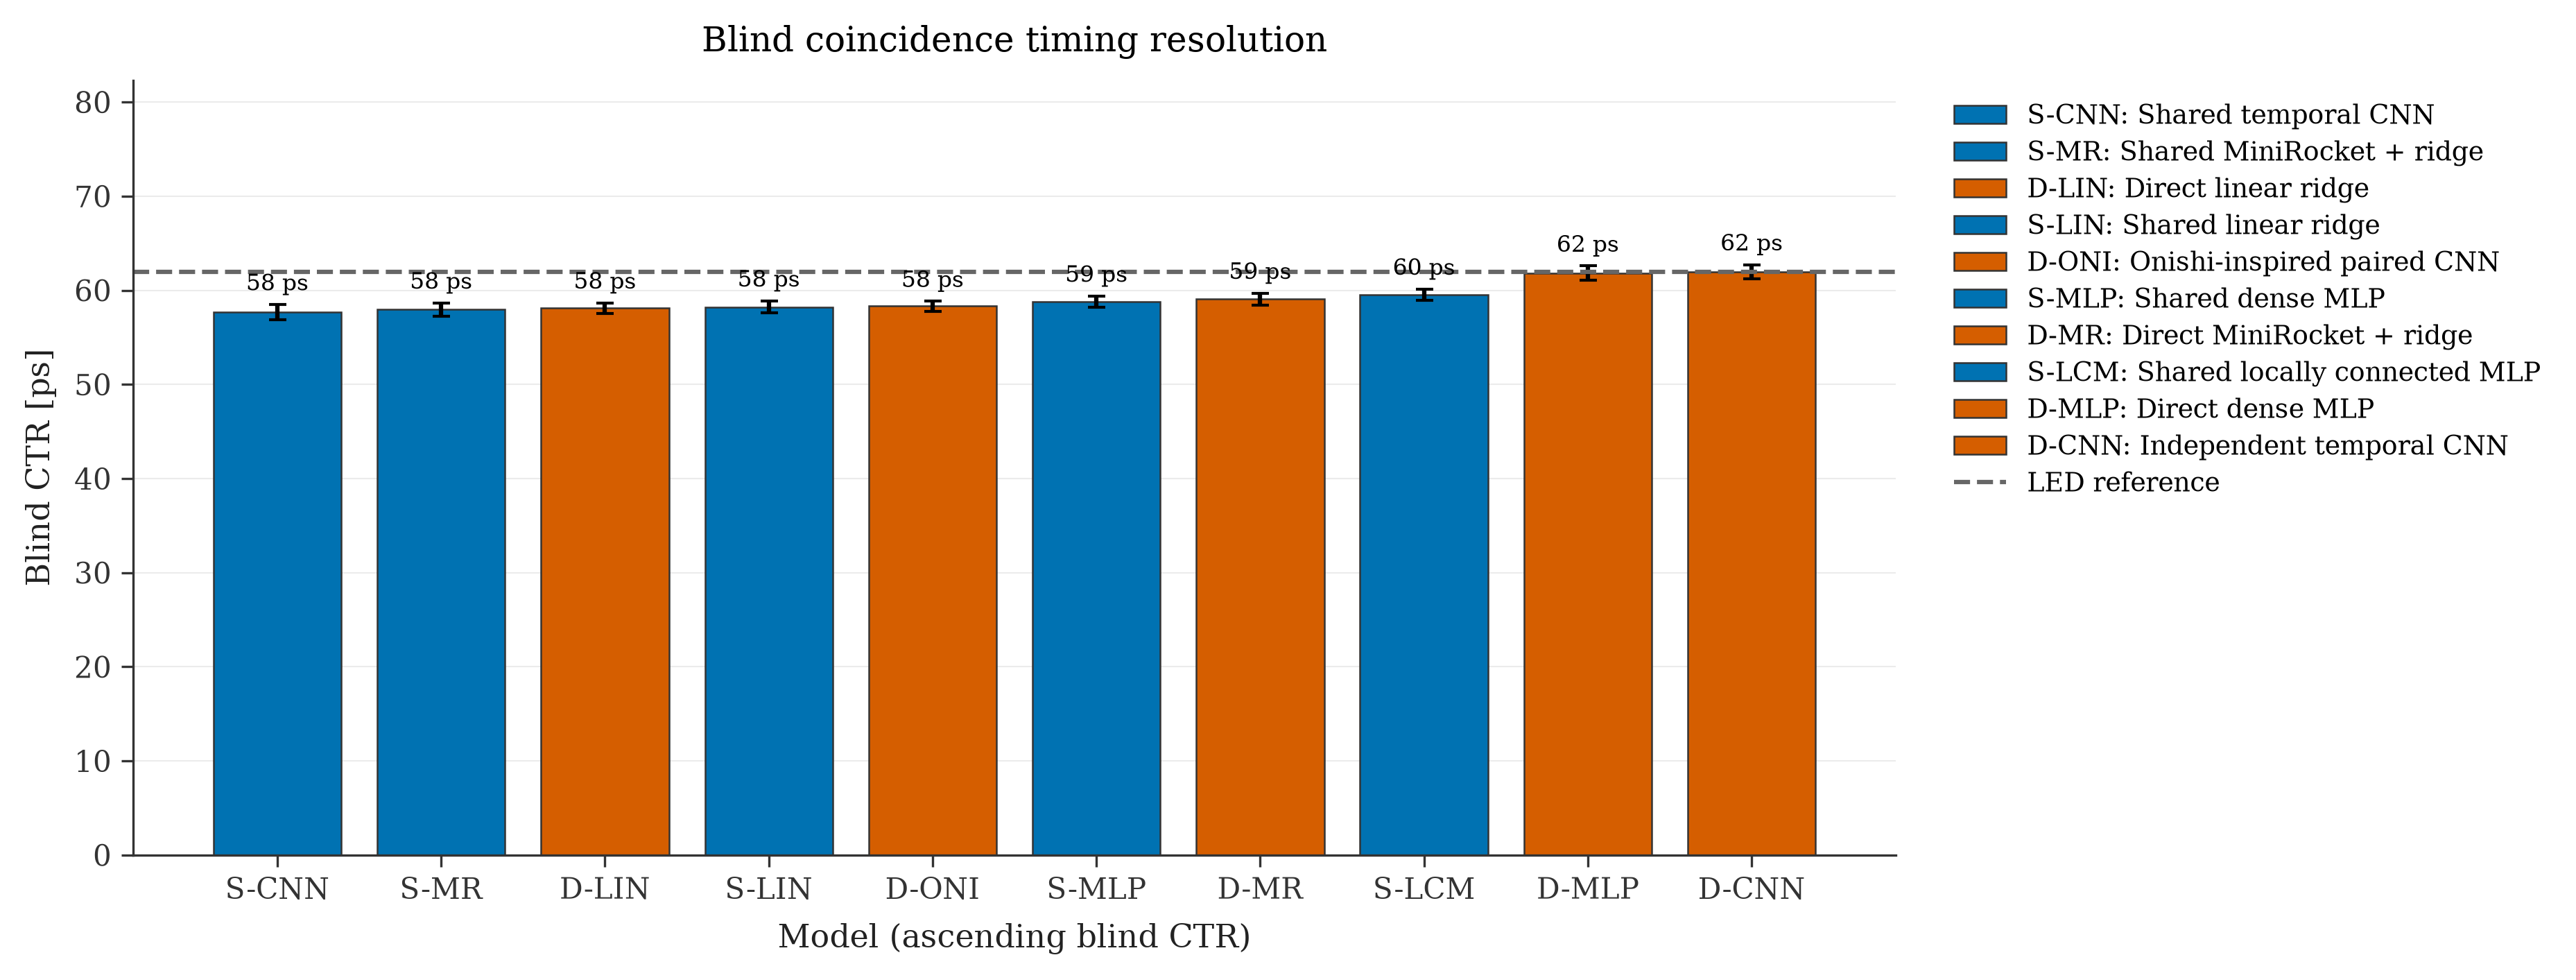
\includegraphics[width=\linewidth]{figures/results/FBK/FBK_timing_onishi_blind_ctr.png}
\caption{Timing, Onishi-inspired window.}
\label{fig:fbk-timing-onishi-ctr}
\end{subfigure}\hfill
\begin{subfigure}[t]{0.49\textwidth}
\centering
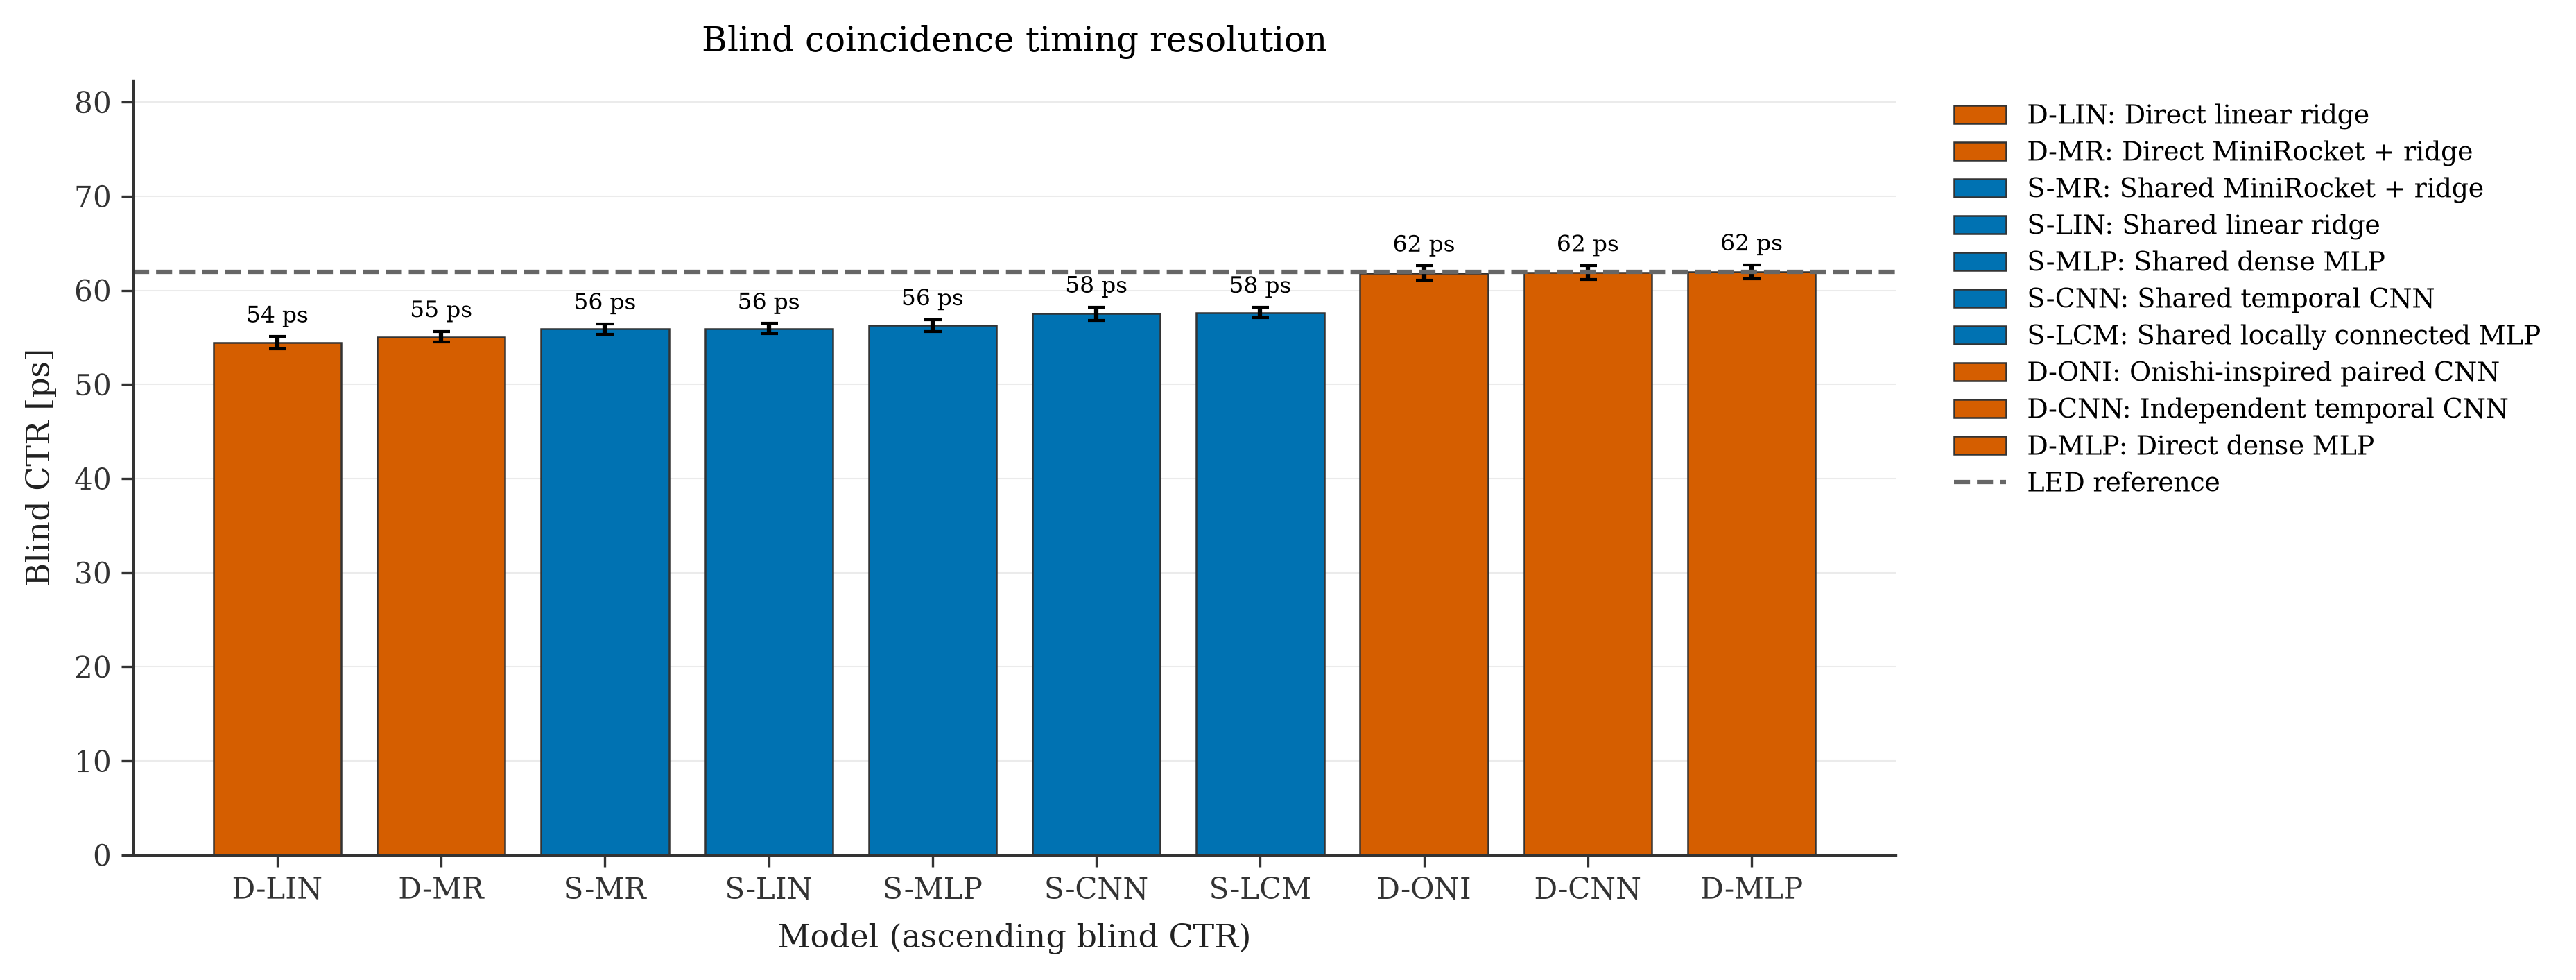
\includegraphics[width=\linewidth]{figures/results/FBK/FBK_timing_wide_blind_ctr.png}
\caption{Timing, wide window.}
\label{fig:fbk-timing-wide-ctr}
\end{subfigure}
\caption{FBK board: independent-test CTR for the compared estimators. The dashed
line denotes the LED reference and error bars indicate bootstrap standard
deviations.}
\label{fig:fbk-ctr-comparison}
\end{figure*}

\FloatBarrier
\bibliographystyle{unsrtnat}
\bibliography{references}
\end{document}
